\documentclass[12pt]{report}
% \documentclass[12pt,twoside]{report} use this to print on both sides
\usepackage[utf8]{inputenc}
\usepackage{setspace}
\usepackage{graphicx}
\usepackage[a4paper,top=25mm,bottom=25mm,left=25mm,right=25mm]{geometry}
\usepackage[dvipsnames]{xcolor}
\usepackage{tocloft}
\usepackage{placeins}
\renewcommand{\cfttoctitlefont}{\hspace*{\fill}\Large\bfseries}
\renewcommand{\cftaftertoctitle}{\hspace*{\fill}}
\renewcommand{\cftlottitlefont}{\hspace*{\fill}\Large\bfseries}
\renewcommand{\cftafterlottitle}{\hspace*{\fill}}
\renewcommand{\cftloftitlefont}{\hspace*{\fill}\Large\bfseries}
\renewcommand{\cftafterloftitle}{\hspace*{\fill}}

\usepackage{sectsty}
\chapternumberfont{\Large}
\chaptertitlefont{\Large}
\usepackage{amsmath}
\usepackage{amssymb}
\usepackage{hyperref}
\usepackage{listings}
\usepackage{verbatim}
\usepackage{array}
\usepackage{float}
\usepackage{caption}
\usepackage{subcaption}
\usepackage{tikz}
\usepackage{everypage}
\usetikzlibrary{shapes.geometric, arrows.meta, positioning}
\usepackage{microtype}
\usepackage{enumitem}
\usepackage{tcolorbox}
\usepackage{newtxtext}
\usepackage{newtxmath}

\AddEverypageHook{
    \ifnum\value{page}>0
    \begin{tikzpicture}[remember picture,overlay]
        \draw[line width=0.8pt]
        ([xshift=0.75cm,yshift=0.75cm]current page.south west)
        rectangle
        ([xshift=-0.75cm,yshift=-0.75cm]current page.north east);
    \end{tikzpicture}
    \fi
}


\pagenumbering{roman}

% This command removes the red border around hyperlinks
\hypersetup{
    colorlinks=true,
    linkcolor=black,
    filecolor=magenta,      
    urlcolor=cyan,
}



% document begins here
\begin{document}
\setlength{\parskip}{0.3cm}
\setstretch{1}
%\setlength{\parskip}{0pt}
\setlength{\parindent}{15pt}

\setlist[itemize]{
    itemsep=1pt,
    topsep=2pt,
    parsep=0pt,
    partopsep=0pt
}
\begin{titlepage}
\thispagestyle{empty}

% --- BACKGROUND ILLUSTRATIONS (TIKZ) ---
% SwiftBite Brand Colors
\definecolor{brandPrimary}{HTML}{14532D}   % Dark Forest Green
\definecolor{brandSecondary}{HTML}{D1E8D5} % Soft Sage/Mint Green
\definecolor{brandText}{HTML}{1F2937}      % Dark Charcoal Typography
\definecolor{brandBg}{HTML}{F4F4F0}        % Warm Off-White 

% \pagecolor{brandBg} % Uncomment this line if you want the off-white background!

\begin{tikzpicture}[remember picture, overlay]

    % Decorative Border
    \draw[brandPrimary, line width=1pt]
    ([xshift=0.5cm,yshift=0.5cm]current page.south west)
    rectangle
    ([xshift=-0.5cm,yshift=-0.5cm]current page.north east);

    \draw[brandPrimary, line width=0.4pt]
    ([xshift=0.8cm,yshift=0.8cm]current page.south west)
    rectangle
    ([xshift=-0.8cm,yshift=-0.8cm]current page.north east);
    
    % Top Right Forest Green Blob (Scaled down to keep text clear)
    \path[fill=brandPrimary] 
        (current page.north east) coordinate (NE)
        (NE) ++(-4.5, 0) coordinate (P1)
        (NE) ++(0, -4.5) coordinate (P2)
        (P1) .. controls ++(2, -0.5) and ++(-1, 1.5) .. (P2) -- (NE) -- cycle;

    % Top Right Sage Green Blob
    \path[fill=brandSecondary] 
        (current page.north east) coordinate (NE2)
        (NE2) ++(-2.5, 0) coordinate (Y1)
        (NE2) ++(0, -2.5) coordinate (Y2)
        (Y1) .. controls ++(1, -1) and ++(-1, 1) .. (Y2) -- (NE2) -- cycle;
        
    % Top Decorative Line & Dots
    
    \fill[brandPrimary] (current page.north east) ++(-1.5,-5.5) circle (0.12);
    \fill[brandSecondary] (current page.north east) ++(-2.5,-3.5) circle (0.18);

    % Bottom Left Forest Green Blob (Scaled down so names are visible)
    \path[fill=brandPrimary, opacity=0.95] 
        (current page.south west) coordinate (SW)
        (SW) ++(3.5, 0) coordinate (P3)
        (SW) ++(0, 4.5) coordinate (P4)
        (P3) .. controls ++(-1.5, 1) and ++(0.5, -2) .. (P4) -- (SW) -- cycle;

    % Bottom Left Sage Green Blob
    \path[fill=brandSecondary] 
        (current page.south west) coordinate (SW2)
        (SW2) ++(2, 0) coordinate (Y3)
        (SW2) ++(0, 2.5) coordinate (Y4)
        (Y3) .. controls ++(-0.5, 1) and ++(1, -0.5) .. (Y4) -- (SW2) -- cycle;
        
    % Bottom Decorative Line & Dots
    
    \fill[brandPrimary] (current page.south west) ++(1.2,5) circle (0.12);
    \fill[brandSecondary] (current page.south west) ++(0.8,3) circle (0.18);
\end{tikzpicture}
% --- END BACKGROUND ---


% --- FOREGROUND TEXT & LOGOS ---
\begin{center}
    \color{brandText} % Applies Dark Charcoal to all text
    
    % NALCO Section
    \vspace*{0.5cm}
    \begin{minipage}{0.2\textwidth}
        \centering
        
\includegraphics[width=\linewidth]{Header/nalco2.jpg}
    \end{minipage}
    
    \vspace{0.3cm}
    {\large \textbf{National Aluminium Company Limited (NALCO)}}\\[0.1cm]
    {\normalsize \textbf{Alumina Refinery Plant, Damanjodi}}\\
    {\small Koraput, Odisha}
    
    \vspace{1.5cm}
    
    % Title Section 
    {\large \textsf{VOCATIONAL TRAINING REPORT}}\\[0.2cm]
    {\normalsize \textsf{ON}}\\[0.4cm]
    {\huge \textbf{\textsf{SwiftBite}}}\\[0.2cm] 
    {\Large \textsf{An Intelligent Food Ordering System}}
    
    \vspace{1.5cm}
    
    % XIM Section
    
\includegraphics[width=0.18\textwidth]{Header/ximlogo.png}
    
    \vspace{0.3cm}
    {\large \textbf{XIM University}}\\[0.1cm]
    {\normalsize School of Computer Science and Engineering}\\
    {\small Bhubaneswar, Odisha, India}
    
    \vspace{0.8cm}
    
    % Training Details
    {\normalsize \textbf{Training Period}}\\
    {\normalsize 02/05/2026 to 31/05/2026}
    
    \vfill 
    
    % Footer Section (Now safely clear of the corner vectors)
    \begin{minipage}[t]{0.48\textwidth}
        \begin{flushleft}
            {\normalsize \textbf{Submitted by:}}\\[0.2cm]
            {\small \textbf{Abhibita Sanya Priyadarshani} \\(Regd No. - RF2026CS0035) \\(University Roll No.- UCSE23001)}
        \end{flushleft}
    \end{minipage}
    \hfill
    \begin{minipage}[t]{0.45\textwidth}
        \begin{flushright}
            {\normalsize \textbf{Under the Guidance of:}}\\[0.2cm]
            {\small \textbf{Dillip Kumar Sahoo}}\\
            {\small Deputy General Manager\\(Systems)}
        \end{flushright}
    \end{minipage}

    

\end{center}
\end{titlepage}

\newpage
\begin{center}

\vspace*{0.5in}

\textbf{SYSTEMS DEPARTMENT} \\
National Aluminium Company Limited (NALCO) \\
Alumina Refinery Plant, Damanjodi\\
Koraput, Odisha. India

\vspace{1cm}

\textbf{\underline{CERTIFICATE}}

\end{center}

\begin{doublespace}

{ This is to certify that the Vocational Training Report titled \textbf{``SwiftBite: An Intelligent Food Ordering System''} submitted by  Abhibita Sanya Priyadarshani (RF2026CS0035) 
of XIM University, Bhubaneswar, in partial fulfilment of the requirements for Vocational Training, is a record of the work carried out by them at \textbf{National Aluminium Company Limited (NALCO), Alumina Refinery Plant, Damanjodi} under the guidance and supervision of the undersigned.}

To the best of my knowledge, this report embodies the original work carried out by the student during the training period and has not been submitted elsewhere for any academic requirement.

\vspace{1.5cm}

\begin{flushleft}
Place: Damanjodi
\hfill
Dillip Kumar Sahoo
\end{flushleft}

\begin{flushleft}
Date: 30/05/26
\hfill
\textbf{Deputy General Manager (Systems)}
\end{flushleft}

\end{doublespace}
\addcontentsline{toc}{chapter}{Certificate}
\newpage
\begin{center}

\textbf{\underline{DECLARATION}}

\end{center}

\vspace{1cm}

\begin{doublespace}

{I Abhibita Sanya Priyadarshani (RF2026CS0035), students of the School of Computer Science and Engineering, XIM University, hereby declare that the Vocational Training Report titled “SwiftBite: An Intelligent Food Ordering System” submitted by us is an original work carried out during our vocational training at \textbf{National Aluminium Company Limited (NALCO), Alumina Refinery Plant, Damanjodi}.

\vspace{0.5cm}

{I further declare that this report has been prepared by me under proper guidance and supervision and has not been copied from any source without appropriate acknowledgement or citation. This work has not previously formed the basis for the award of any Degree, Diploma, Fellowship, or any other similar recognition.}

\vspace{1.2cm}

\begin{flushleft}
Place: Damanjodi
\hfill
Abhibita Sanya Priyadarshani (RF2026CS0035)
\begin{flushleft}
Date: 30/05/26
\end{flushleft}

\end{doublespace}
\addcontentsline{toc}{chapter}{Candidate's Declaration}
\newpage
\begin{center}

\vspace{1cm}

\textbf{\underline{ACKNOWLEDGEMENT}}

\end{center}

\vspace{1cm}

\begin{doublespace}

I would like to express my sincere gratitude to 
\textbf{National Aluminium Company Limited (NALCO), Alumina Refinery Plant, Damanjodi} 
for providing us the opportunity to undergo vocational training at their esteemed organization.

I am deeply thankful to 
\textbf{Mr. Dillip Kumar Sahoo, Deputy General Manager (Systems)}, 
for his valuable guidance, constant support, and encouragement throughout the training period. His insights and suggestions greatly helped me in understanding the practical applications and industrial relevance of the project titled 
\textbf{``SwiftBite: An Intelligent Food Ordering System''}.

I also extend our heartfelt thanks to the officials and staff members of the Systems Department at NALCO for their cooperation and assistance during the course of our training.

Finally, I express my gratitude to the faculty members of the School of Computer Science and Engineering, XIM University, for their continuous encouragement and support.

\vspace{1cm}

\begin{flushleft}
Place: Damanjodi
\hfill
Abhibita Sanya Priyadarshani
\begin{flushleft}
Date: 30/05/26
\end{flushleft}



\end{doublespace}
\addcontentsline{toc}{chapter}{Acknowledgement}
\newpage
\begin{center}

\vspace*{0.3in}

\Large{\textbf{Abstract}}

\vspace{5mm}

\end{center}

\justifying

SwiftBite is a web-based food-ordering prototype developed to demonstrate a customer ordering experience alongside role-specific portal interfaces and a supporting backend API. The frontend is built with React, TypeScript, and Vite. It includes a landing page, account registration and login screens, restaurant and menu browsing, a shopping cart, checkout, order-status screens, and profile features.

\vspace{0.5cm}

The customer storefront currently uses bundled sample restaurant and menu data. Cart, checkout, and order-status interactions are demonstrations and do not yet create persistent orders or process payments. The delivery screen loads OpenStreetMap tiles centered on Bhubaneswar with zoom controls, but its city-center marker and order timeline are demonstrations rather than live rider tracking. The frontend communicates with the backend for account registration and login and for chatbot assistance. The Express and TypeScript backend exposes additional API routes for restaurants, profiles, menu items, uploads, orders, dashboards, and chatbot requests. The backend is connected to MySQL: the eight-table schema was initialized, four restaurants and four categories were seeded, and the restaurant API was verified to return database-backed records. Authentication retains a file-backed fallback if database operations fail.

\vspace{0.5cm}

The backend Gemini integration successfully generated a recipe response during chatbot testing, as shown in the results section. It retries transient primary-model failures, tries a secondary model if the primary fails, and retains a local rule-based response path if Gemini is unavailable. The chatbot does not access live order data or place orders. The admin, restaurant-owner, and delivery-partner portals are demonstration interfaces and are not protected by complete server-side role authorization.

\vspace{5mm}

\noindent\textbf{Keywords}

\noindent Food Ordering Prototype, React, TypeScript, Vite, Express.js, MySQL, User Authentication, Chatbot, Web Application


\addcontentsline{toc}{chapter}{Abstract}
\newpage
\begin{center}

\vspace*{0.3in}

\Large{\textbf{Project Objective}}

\vspace{5mm}

\end{center}

\justifying

The objective of \textbf{``SwiftBite: An Intelligent Food Ordering System''} is to design and develop a web-based prototype that demonstrates the main screens and supporting services of an online food-ordering application.

\vspace{5mm}

\begin{itemize}
    \item To build a responsive customer interface for browsing sample restaurants and menus, managing a cart, and viewing checkout and order-status screens.
    \item To provide account registration and login screens with email or phone selection and password-confirmation validation.
    \item To develop a separate Express API for authentication, restaurant and profile data, menu items, uploads, orders, dashboards, and chatbot assistance.
    \item To provide a MySQL schema and configurable database connection for backend persistence.
    \item To demonstrate app-guidance chatbot responses using local fallback behavior and optional Gemini integration.
    \item To illustrate customer, administration, restaurant-owner, and delivery-partner workflows while clearly identifying demo-only features.
\end{itemize}


\addcontentsline{toc}{chapter}{Project Objective}
\newpage
\begin{center}

\Large{\textbf{Technology Used}}

\vspace{5mm}

\end{center}

\justifying

The SwiftBite prototype uses a React and TypeScript frontend, a Node.js and Express backend, and a working MySQL database connection. The database connection, initialized schema, and restaurant API have been verified.

\vspace{3mm}

\textbf{Frontend Technologies}
\begin{itemize}
    \item \textbf{React 19} -- Used to build the user interface from reusable components.
    \item \textbf{Vite} -- Used as the frontend development server and production build tool.
    \item \textbf{TypeScript} -- Used for typed frontend code.
    \item \textbf{Tailwind CSS 4 and custom CSS} -- Used for utility styling, layouts, and responsive presentation.
    \item \textbf{Web App Manifest and Service Worker} -- Included for installable web-app support.
\end{itemize}

\vspace{3mm}

\textbf{Backend and Data Technologies}
\begin{itemize}
    \item \textbf{Node.js, Express 5, and TypeScript} -- Used to implement the backend HTTP API.
    \item \textbf{MySQL and mysql2} -- Used by the backend for relational storage; the connection and schema are verified, and the restaurant API reads records from MySQL.
    \item \textbf{Zod} -- Used to validate authentication, chatbot, and other request payloads.
    \item \textbf{CORS and Helmet} -- Used for cross-origin configuration and HTTP security headers.
    \item \textbf{Morgan and Dotenv} -- Used for HTTP request logging and environment-variable configuration.
    \item \textbf{Google Generative AI SDK} -- Connects the backend chatbot to Gemini. The configured primary model is \texttt{gemini-3.8-flash}; transient HTTP 429 and 5xx failures receive one retry with exponential backoff and jitter, followed by one attempt using \texttt{gemini-3.6-flash}. A local rule-based response remains available if model generation fails. A generated recipe response was verified during testing; the API key is supplied server-side and is not included in this report.
\end{itemize}

\vspace{3mm}

\textbf{Development Tools}
\begin{itemize}
    \item Visual Studio Code (VS Code)
    \item Git and GitHub
    \item npm
\end{itemize}


\addcontentsline{toc}{chapter}{Technology Used}
\newpage
\begin{center}

\Large{\textbf{Key Features of the Project}}

\vspace{5mm}

\end{center}

\justifying

\begin{itemize}

    \item \textbf{Customer-Facing Food Ordering Prototype}
    The web interface demonstrates restaurant browsing, menu details, category filtering, favourites, and cart quantity changes using bundled sample data.
    \vspace{0.3cm}

    \item \textbf{Account Registration and Login}
    Registration accepts an email address or phone number and includes required password confirmation. Authentication requests are sent to the backend API.
    \vspace{0.3cm}

    \item \textbf{Checkout and Order-Status Screens}
    The frontend presents delivery, payment-selection, checkout, confirmation, and order-status screens. Place Order opens a confirmation screen, from which Track My Order opens a zoomable OpenStreetMap view centered on Bhubaneswar. The marker and timeline are demonstrations; payment and order creation are not connected to a live transaction workflow.
    \vspace{0.3cm}

    \item \textbf{Demonstration Portals}
    Customer, admin, restaurant-owner, and delivery-partner views illustrate different workflows. Portal switching is explicitly marked as demo functionality and does not provide production role authorization.
    \vspace{0.3cm}

    \item \textbf{Chatbot Assistance}
    The backend chatbot uses Gemini to generate responses; a recipe response was verified during testing. It retries transient primary-model errors and tries a secondary model before using the local rule-based fallback. The server-side API key is not exposed to the frontend.
    \vspace{0.3cm}

    \item \textbf{Backend API and Database Schema}
    The Express API includes routes for authentication, restaurants, profiles, menus, image uploads, orders, dashboards, and chatbot assistance. Its MySQL database is connected and initialized; the restaurant API has been verified to read database records.
    \vspace{0.3cm}

    \item \textbf{Responsive Web-App Experience}
    The React interface is designed for desktop and mobile layouts and includes a web app manifest and service-worker registration.

\end{itemize}


\addcontentsline{toc}{chapter}{Key Features}
\newpage
\setcounter{tocdepth}{2}
\addcontentsline{toc}{chapter}{Content}
\tableofcontents

\newpage


\input{Header/symbol}

% CHAPTERS BEGIN
\pagenumbering{arabic}
\chapter{Introduction about NALCO}

National Aluminium Company Limited (NALCO) is one of the leading public sector enterprises in India engaged in the production of alumina and aluminium. Established in the year 1981, NALCO operates under the Ministry of Mines, Government of India, and is recognized as one of the largest integrated Bauxite-Alumina-Aluminium-Power complexes in the country. The company plays a major role in India’s aluminium industry through its mining, refining, smelting, and power generation operations.

As a globally recognized Navratna Central Public Sector Enterprise (CPSE), NALCO is renowned for its operational excellence and financial performance. Its integrated complex manages every stage of production from raw material extraction to the final product. The strategic planning and corporate governance that drive this vast operation originate from its central headquarters in Bhubaneswar.

\begin{figure}[!ht]
    \centering
    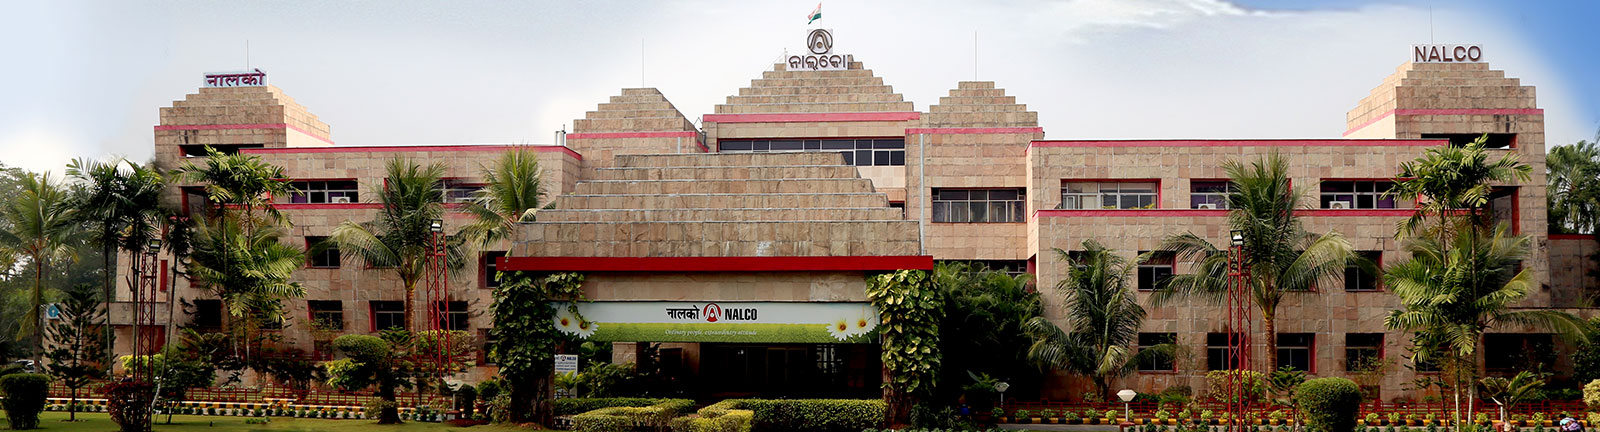
\includegraphics[width=1.0\textwidth]{nalco-corporate office.jpg}
    \caption{NALCO's Corporate Office in Bhubaneswar, serving as the administrative nerve center.}
    \label{fig:corporate}
\end{figure}

The distinct architectural form of NALCO's corporate office building serves as the administrative nerve center. This structure reflects the company's strong industrial presence and oversees the entire spectrum of its diverse operations across multiple locations, ensuring NALCO's position as a globally competitive enterprise and its sustained contribution to India's industrial growth.

\FloatBarrier
\section{Panchpatmali Bauxite Mines}

The first vital link in NALCO's integrated chain is the extraction of raw material. NALCO operates the Panchpatmali Bauxite Mines, located near Damanjodi, which serve as the primary source of bauxite ore. These mines are highly mechanized and rank among the largest open-cast bauxite mines in Asia. The mining operations follow modern techniques and rigorous environmental conservation measures to ensure sustainable practices.

\begin{figure}[!ht]
    \centering
    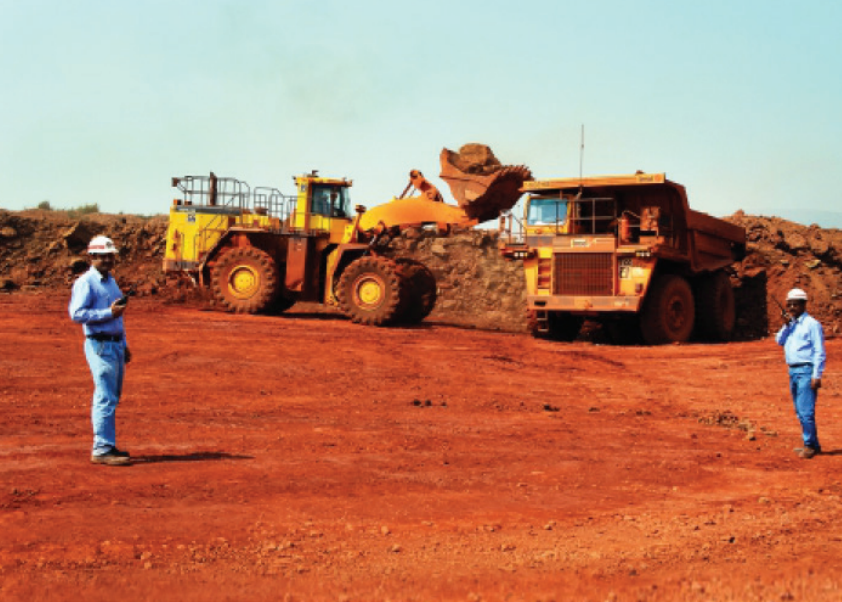
\includegraphics[width=0.8\textwidth]{Chapters/bauxitemine.png}
    \caption{Heavy machinery operating at the Panchpatmali Bauxite Mines.}
    \label{fig:mines}
\end{figure}

The continuous and efficient operation of these mines relies heavily on advanced heavy earth-moving machinery. The scale of this mechanized extraction is clearly visible in the rich, red terrain of the mine. Personnel oversee massive front-end loaders and heavy-duty dump trucks working systematically to extract and load the bauxite ore for transport.

\FloatBarrier
\section{NALCO Alumina Refinery, Damanjodi}

Following the initial mining process, the bauxite ore is transported to the Alumina Refinery located at Damanjodi in the Koraput district of Odisha. This refinery processes the bauxite ore into alumina through the specialized Bayer Process, serving as a critical bridge in NALCO's value chain.

\begin{figure}[!ht]
    \centering
    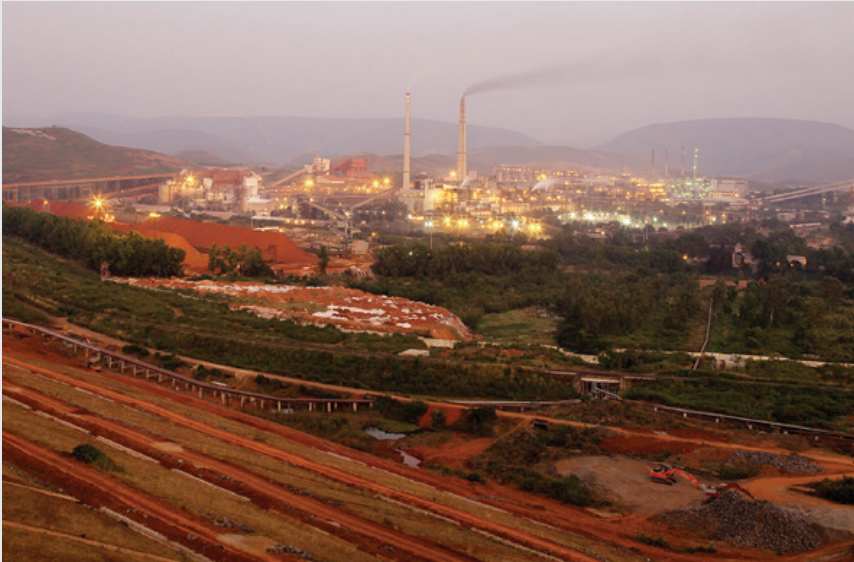
\includegraphics[width=0.8\textwidth]{Chapters/aluminarefinary.png}
    \caption{Dusk view of the sprawling NALCO Alumina Refinery at Damanjodi.}
    \label{fig:refinery}
\end{figure}

The Damanjodi refinery is equipped with advanced process control systems, extensive bauxite handling facilities, and vast chemical processing units, including multiple calcination kilns. The sprawling nature of this refinery, nestled against a backdrop of rolling hills, is captured dramatically at dusk with its extensive network of illuminated processing plants and operational smokestacks.

\FloatBarrier
\section{Captive Power Plant}

Aluminium production is an incredibly energy-intensive process, specifically during the smelting stage. To ensure an economical and uninterrupted supply of electricity, NALCO operates a massive dedicated Captive Power Plant. This thermal power facility guarantees the company's energy security and competitive operational independence.

\begin{figure}[!ht]
    \centering
    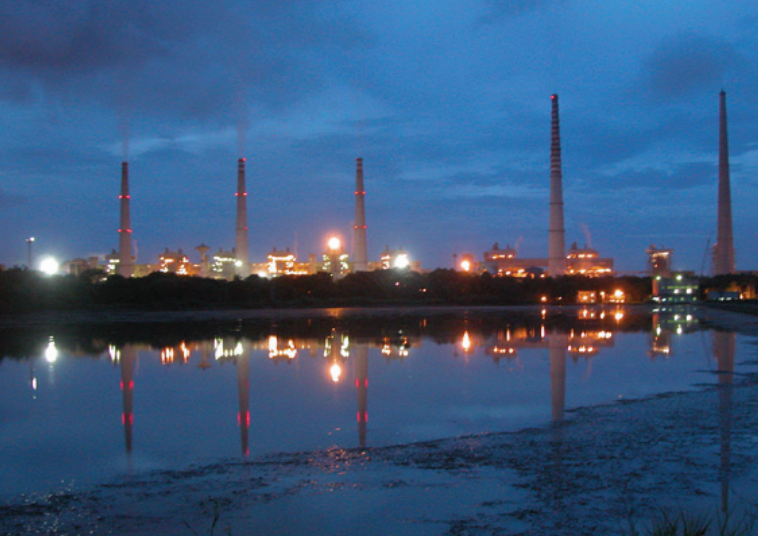
\includegraphics[width=0.8\textwidth]{Chapters/captivepowerplant.png}
    \caption{The illuminated Captive Power Plant ensuring uninterrupted energy supply.}
    \label{fig:powerplant}
\end{figure}

The striking profile of this critical power generation complex is shown brilliantly illuminated against the evening sky. The towering smokestacks and cooling infrastructure of the plant are reflected clearly over the adjacent body of water, illustrating its substantial scale and continuous operation.

\FloatBarrier
\section{Aluminium Smelter Complex}

The pure alumina refined at Damanjodi and the reliable power generated by the captive plant come together at NALCO’s large-scale aluminium smelter. This complex is where the actual production of metal occurs, using an electrolytic process to convert alumina into high-grade molten aluminium, which is then cast into various commercial forms.

\begin{figure}[!ht]
    \centering
    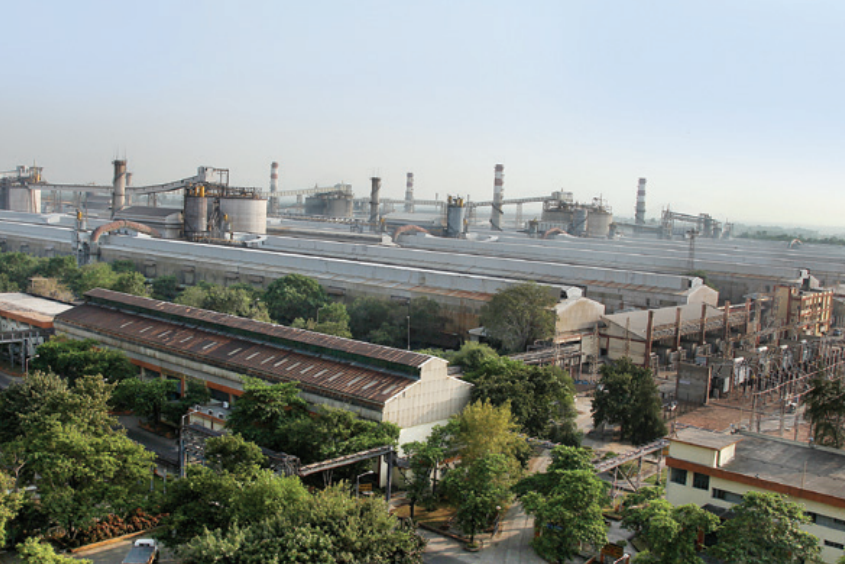
\includegraphics[width=0.8\textwidth]{Chapters/smelter.png}
    \caption{Aerial layout of the massive Aluminium Smelter Complex.}
    \label{fig:smelter}
\end{figure}

The sheer scale and meticulous industrial organization of the smelting facility are highly distinctive. The elevated perspective illustrates the sprawling, grid-like layout of the plant, dominated by exceptionally long, parallel industrial buildings that house the specialized potlines where electrolysis takes place.

\FloatBarrier
\section{Renewable Energy and Sustainability}

Beyond its traditional heavy industrial operations, NALCO is deeply committed to sustainable development and environmental conservation. As a forward-thinking Navratna CPSE, the company actively implements eco-friendly mining practices, waste management systems, extensive afforestation programs, and community development initiatives in its surrounding areas.

\begin{figure}[!ht]
    \centering
    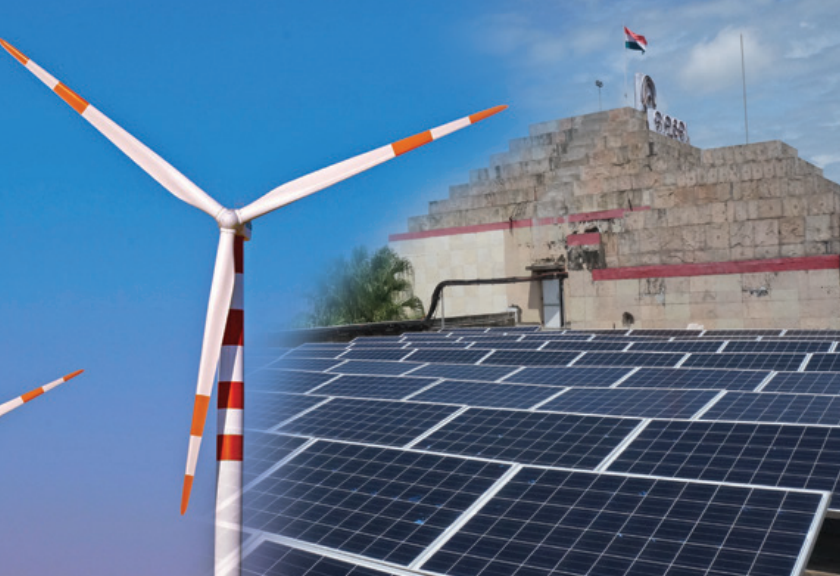
\includegraphics[width=0.8\textwidth]{Chapters/wind_solar.png}
    \caption{NALCO's renewable energy infrastructure including wind turbines and solar panels.}
    \label{fig:renewables}
\end{figure}

Embracing a future of clean energy, NALCO has made significant investments in renewable power sources, adding wind power plants and solar installations to its portfolio. This proactive pivot toward sustainability is visually represented by modern, high-capacity wind turbines working in tandem with a broad array of rooftop solar panels, symbolizing the company's dual commitment to clean industrial energy and traditional operations.


\chapter{Introduction about the IT Department}

The Information Technology (IT) Department at National Aluminium Company Limited (NALCO) plays a crucial role in managing and supporting the organization’s digital infrastructure, communication systems, enterprise applications, and industrial information systems. As a large integrated public sector enterprise with operations spread across mines, refinery units, smelter plants, power plants, and corporate offices, NALCO relies heavily on robust IT systems to ensure smooth coordination, secure data management, and efficient industrial operations.

The IT Department is responsible for maintaining the organization’s computer networks, servers, databases, enterprise software systems, and cybersecurity infrastructure. It supports the automation and digitalization of various administrative, operational, and industrial processes across different units of the organization. The department ensures uninterrupted connectivity and communication between operational locations such as Damanjodi, Angul, Bhubaneswar, and other regional offices.

One of the major responsibilities of the IT Department is the management of enterprise-level software systems used for finance, human resources, inventory management, procurement, payroll, production monitoring, and reporting operations. These systems help streamline organizational workflows, improve operational efficiency, and support data-driven decision making across departments.

The department also manages network infrastructure including Local Area Networks (LAN), Wide Area Networks (WAN), internet services, firewall systems, VPN connectivity, and secure communication channels. Regular monitoring, maintenance, troubleshooting, and system updates are carried out to ensure network reliability and data security within the organization.

Another important function of the IT Department is data management and backup administration. Large volumes of operational and administrative data generated across different NALCO units are securely stored, monitored, and maintained through centralized database systems and backup procedures. The department follows standard data security protocols, access control mechanisms, and disaster recovery procedures to protect critical organizational information from unauthorized access or system failures.

The IT Department also plays a significant role in maintaining industrial automation support systems and process monitoring applications used in refinery and mining operations. These systems assist in monitoring plant operations, production activities, equipment status, and process parameters in real time, thereby improving operational control and efficiency.

\section{Data Centre Facilities}

NALCO’s IT infrastructure includes dedicated data centre facilities that support centralized storage, processing, and management of organizational data and applications. The data centre contains servers, storage devices, networking equipment, backup systems, and security mechanisms required for running enterprise applications and maintaining uninterrupted digital operations.

The data centre environment is designed with proper cooling systems, uninterrupted power supply (UPS), backup generators, and physical security controls to ensure continuous system availability and protection of critical hardware infrastructure. The servers hosted within the data centre support database management systems, enterprise resource planning (ERP) applications, internal portals, email services, and other operational software used across the organization.

Regular data backup procedures, server monitoring, software updates, and cybersecurity measures are implemented within the data centre to ensure secure and reliable system performance. Disaster recovery mechanisms and redundancy systems are also maintained to minimize downtime and ensure business continuity during technical failures or emergencies.

\section{Procedures and Workflow Management}

The IT Department follows structured procedures for managing technical support, software maintenance, user access control, and system administration. User requests and technical issues are handled through organized support and troubleshooting processes to ensure minimal disruption in organizational operations.

Software updates, security patches, system maintenance, and database monitoring are performed regularly to maintain system stability and security. Access permissions are managed based on user roles and departmental requirements to ensure controlled access to sensitive organizational data and applications.

The department also coordinates with different operational units and departments to implement new technologies, improve digital infrastructure, and support modernization initiatives within the organization. Through continuous monitoring, maintenance, and technological support, the IT Department contributes significantly to the efficient functioning of NALCO’s industrial and administrative operations.

\section{In-House Mobile Applications and Portals}

The IT and System Department at NALCO has developed a robust suite of in-house mobile applications and digital portals to streamline enterprise workflows, enhance employee engagement, and improve customer relations. These applications ensure that critical operational data and services are securely accessible on the go.

\begin{itemize}
    \item \textbf{NALCO Netra:} A unified mobile application designed to provide active employees with convenient access to key information and self-service transactions, including payroll, attendance, and leave management.
    
    \item \textbf{NALCO Sanjeevani:} A dedicated family wellness and child care app designed specifically for employees and associated families, providing comprehensive health resources and support.
    
    \item \textbf{NISARG:} (Nalco Initiatives for Social Awareness and Responsible Growth) A mobile app that highlights the company's Corporate Social Responsibility (CSR) efforts, showcasing social impact projects and annual reports.
    
    \item \textbf{Hamesha Nalconian:} A dedicated portal for retired NALCO employees, serving as a single point for information on post-retirement medical reimbursements, empaneled hospitals, and related corporate policies.
    
    \item \textbf{NAGINAA:} (Nalco Grahak Information and Networking App for All) A customer-focused application providing details about products, pricing, MOU schemes, and dispatch information.
    
    \item \textbf{NAMASYA:} (Nalco Micro And Small enterprise Yogayog Application) An application tailored for MSE vendors to access registration processes, technical specifications, and vendor development programs.
    
    \item \textbf{Nalco Suraksha:} A mobile app utilized for on-site safety inspection reporting, instantly recording fire hazards, first aid requirements, and unsafe conditions at plant locations.
    
    \item \textbf{NALCO Smart Township:} An application developed for NALCO township residents and employees to raise property maintenance calls and seamlessly manage the Gate Pass system.
\end{itemize}
\chapter{Project Introduction}

The rapid growth of online food delivery services has significantly transformed the way customers order and access food in modern lifestyles. With increasing dependence on digital platforms, users now expect fast, convenient, and personalized food ordering experiences.

\vspace{0.5mm}

Traditional food ordering systems primarily focus on basic order placement and delivery functionalities, often lacking intelligent interaction, personalized recommendations, and efficient management features. As competition in the food delivery industry continues to increase, there is a growing need for a smart and scalable system that can improve customer experience while simplifying restaurant and delivery operations.

\vspace{0.5mm}

The SwiftBite project explores these challenges through a web-based food-ordering prototype with a customer storefront, account flows, and demonstration portals for different user roles. It also provides chatbot assistance for common application questions. The prototype combines a React frontend with a backend API connected to MySQL; the database connection and restaurant API have been verified. Persistent ordering, payment processing, and production role authorization remain areas for further development.

\section{Project Objectives}

The primary objective of the SwiftBite project is to develop and evaluate a user-friendly food-ordering prototype with an account flow, a customer storefront, and illustrative interfaces for customer, restaurant, delivery, and administration workflows.

The project also includes chatbot assistance for application questions. A Gemini-generated recipe response was verified during testing; transient primary-model failures are retried and a secondary model is attempted before local rule-based guidance is used. The chatbot is not a personalized recommendation engine.

The project uses a React, TypeScript, and Vite frontend with a Node.js and Express API and a MySQL schema. The customer restaurant catalogue, cart, checkout, and tracking screens are currently prototype flows, rather than a complete real-time ordering and delivery service.

\section{Background of the Project}

The inspiration for SwiftBite arises from the demand for convenient online food-ordering experiences. The prototype explores this area through a customer-facing interface, account flows, and application guidance from a chatbot. It does not analyze customer preferences or generate personalized food recommendations.

The current implementation uses React and Vite for the frontend, an Express API for backend services, and a connected MySQL database with an initialized schema. The backend restaurant endpoint has been verified against MySQL. The backend Gemini integration returned a generated response during chatbot testing, with transient-error retry, a secondary model, and local rule-based guidance as fallback layers. The customer storefront still uses bundled catalogue data. Checkout and order status are demonstrations; the delivery screen provides a zoomable OpenStreetMap view centered on Bhubaneswar with a static marker. Persistent customer orders, payment processing, live rider tracking, personalized recommendations, and production access control remain future work.

\section{Operation Environment}

The SwiftBite application operates as a web-based prototype. The frontend is developed using \textbf{React}, \textbf{TypeScript}, and \textbf{Vite}, with \textbf{Tailwind CSS} and custom CSS for its responsive interface. The project also includes a web app manifest and service-worker registration.

The backend is developed using \textbf{Node.js}, \textbf{Express}, and \textbf{TypeScript}. It exposes REST API routes for authentication, restaurant and profile data, menu items, image uploads, orders, dashboards, and chatbot assistance. The backend is connected to \textbf{MySQL} through \texttt{mysql2}; its schema is initialized, and the restaurant API has been verified against the database. The frontend storefront currently uses bundled sample restaurant and menu data, and checkout does not persist orders or payment transactions.

Backend libraries include \textbf{CORS}, \textbf{Helmet}, \textbf{Morgan}, \textbf{Dotenv}, \textbf{mysql2}, and \textbf{Zod}. The chatbot uses the Google Generative AI SDK through a server-side key; local responses remain a fallback when Gemini is unavailable. Role-specific portal switching is marked as a demonstration feature, not production access control.
\input{Chapters/objectives}
\chapter{Literature Review}

\section{Online Food Ordering Systems}

Online food ordering systems have significantly transformed the food service industry by providing customers with convenient access to restaurants and food delivery services through digital platforms. These systems enable users to browse menus, place orders, make online payments, and track deliveries in real time. Popular platforms such as Swiggy and Zomato have demonstrated the effectiveness of centralized food ordering applications in improving customer convenience and restaurant operations. However, many conventional systems mainly focus on basic ordering functionalities and often lack intelligent interaction and personalized user experiences.

These systems provide context for SwiftBite's prototype, which demonstrates restaurant and menu browsing alongside account and chatbot interfaces. Personalized recommendations and NLP-based recommendation features are not implemented.

\section{AI-Powered Chatbot Systems}

AI-powered chatbot systems have become increasingly popular in modern web applications for providing automated customer support and real-time assistance. These systems utilize Natural Language Processing (NLP) techniques to understand user queries and generate human-like responses. Chatbots improve user engagement, reduce response time, and minimize dependency on manual support services.

Existing chatbot systems are widely used in e-commerce, healthcare, banking, and food delivery platforms. SwiftBite provides application guidance through a local rule-based response path and can use Gemini through the backend when configured. It does not provide live order support or place orders through chat.

\section{Recommendation Systems}

Recommendation systems play a major role in enhancing user engagement and personalization in digital platforms. These systems analyze user behavior, search history, and preferences to suggest relevant products or services. In food delivery applications, recommendation systems help customers discover restaurants and food items based on their interests and previous orders.

Many existing food delivery platforms use recommendation algorithms to improve customer satisfaction and increase sales. SwiftBite does not currently implement personalized recommendations; this remains a possible future enhancement.

\section{Role-Based Management Systems}

Role-based access control systems are widely used in modern applications to ensure secure and organized management of multiple user categories. Such systems provide separate interfaces and permissions for administrators, customers, delivery personnel, and service providers.

Food delivery platforms commonly use role-based dashboards for handling restaurant management, delivery tracking, and customer operations efficiently. SwiftBite includes role-specific demonstration views for customers, restaurant owners, delivery personnel, and administrators. These views are not protected by complete server-side role authorization.

\section{Full-Stack Web Development Technologies}

Modern food ordering applications rely heavily on full-stack web technologies to provide scalable, responsive, and efficient user experiences. Frontend frameworks such as React.js and Next.js are widely used for building interactive user interfaces, while backend technologies like Node.js and Express.js are commonly used for handling APIs and business logic.

Database management systems such as MySQL play an important role in storing user information, restaurant details, and order data. SwiftBite's frontend uses React, TypeScript, Vite, Tailwind CSS, and custom CSS; its backend uses Node.js, Express, and TypeScript with a working MySQL connection and initialized schema. The restaurant API has been verified against the database. The customer storefront still uses bundled sample data and is not integrated with persistent order processing.

\section{Application Security and Validation Systems}

Security and validation mechanisms are essential components of modern web applications, especially in systems involving online transactions and user data management. Backend libraries and middleware such as Helmet, CORS, and Zod are commonly used to improve API security, handle cross-origin requests, and validate incoming data.

Logging and monitoring tools like Morgan help developers track API activities and system performance. SwiftBite includes Morgan, CORS, Helmet, and Zod for request logging, cross-origin configuration, security headers, and payload validation. Their presence does not imply complete production security or authorization.

\section{Comparison with Existing Systems}

Many existing food ordering platforms mainly focus on order placement and delivery functionalities, with limited emphasis on intelligent interaction and personalized assistance. Some systems provide recommendation features, while others focus on chatbot integration independently.

SwiftBite combines a customer-facing interface, demonstration portal views, backend API routes, and optional chatbot integration in a prototype. Personalized recommendations, persistent customer ordering, payment processing, live delivery tracking, and production role authorization are not part of the current implementation.
\chapter{System Analysis}

\section{Software Requirement Specification}

The current SwiftBite deliverable is a web prototype that demonstrates customer-facing ordering screens and a supporting API. Its implemented scope is distinguished below from production integrations that remain future work.

\begin{itemize}

\item \textbf{Frontend:} The application must provide a responsive web interface for the landing page, account flows, restaurant and menu browsing, cart, checkout, order-status screens, profile, and demonstration portals.

\item \textbf{Authentication:} The registration and login screens must accept an email address or phone number. Registration requires a name, a password of at least six characters, password confirmation, and acceptance of the terms. The frontend calls the backend authentication endpoints; complete session-token and production authorization flows are not implemented.

\item \textbf{Backend API:} The Express service provides routes for authentication, restaurants, rider and restaurant profiles, menu items, image uploads, orders, dashboards, and chatbot assistance.

\item \textbf{Data:} The backend includes an initialized MySQL schema for users, restaurants, profiles, menu items, uploaded images, and orders. The MySQL connection and restaurant API were verified. The customer storefront currently displays bundled sample restaurant and menu data.

\item \textbf{Ordering:} The frontend demonstrates cart, checkout, and order-status screens. Creating a persistent order, processing a payment, and live GPS tracking are not part of the current customer workflow.

\item \textbf{Delivery Map:} The order screen displays OpenStreetMap tiles centered on Bhubaneswar with zoom controls and an approximate static city-center marker. It does not show a rider's live location.

\item \textbf{Chatbot:} The assistant provides app guidance through the backend Gemini integration when configured, with local responses retained as a fallback. A Gemini-generated recipe response was verified during testing.

\item \textbf{Chatbot Reliability:} The primary model receives one retry for transient HTTP 429 or 5xx errors. If primary generation fails, the backend attempts a secondary model; local rule-based replies remain available if model generation still fails.

\item \textbf{Validation:} Backend request payloads are validated with Zod. The registration flow checks required fields and password confirmation in the frontend and backend.

\end{itemize}

\section{Software Tools Used}

\begin{itemize}

\item \textbf{Frontend:} React 19, TypeScript, Vite, Tailwind CSS 4, and custom CSS.

\item \textbf{Backend:} Node.js, Express 5, and TypeScript.

\item \textbf{Database:} MySQL with the \texttt{mysql2} promise client; the backend is connected and the schema is initialized. The restaurant API is verified. The API also has a file-backed authentication fallback when database operations fail.

\item \textbf{Validation and middleware:} Zod, CORS, Helmet, Morgan, and Dotenv.

\item \textbf{Chatbot integration:} Google Generative AI SDK for Gemini responses; local rule-based responses provide a fallback path.

\item \textbf{Development and version control:} VS Code, npm, Git, and GitHub.

\end{itemize}

\chapter{System Design}

\section{Overview}

SwiftBite is organized as a React frontend and a separate Express API. The frontend uses bundled sample data for the customer restaurant and menu screens and local application state for cart and order-status demonstrations. It calls the backend for account registration and login and chatbot assistance. The backend also exposes routes for restaurant, profile, menu, image-upload, order, and dashboard operations.

The backend is connected to MySQL using environment-based settings. The eight-table schema has been initialized, including four seeded restaurants and four categories, and the database-backed restaurant API has been verified. Authentication retains a file-backed fallback for cases where database operations fail. Portal switching in the frontend is explicitly a demonstration flow; it does not by itself provide server-side role authorization.

\section{Table Design}

\begin{table}[H]
\centering
\caption{Users Table Schema}
\label{tab:users}
\begin{tabular}{|l|l|p{7cm}|}
\hline
\textbf{Field Name} & \textbf{Data Type} & \textbf{Description} \\ \hline
\texttt{id} & BIGINT UNSIGNED & Auto-incrementing primary key \\ \hline
\texttt{full\_name} & VARCHAR(120) & User's display name \\ \hline
\texttt{identifier} & VARCHAR(191) & Email address or phone identifier \\ \hline
\texttt{role} & ENUM & One of \texttt{customer}, \texttt{delivery}, \texttt{restaurant}, or \texttt{platform} \\ \hline
\texttt{password\_hash} & CHAR(64) & SHA-256 password digest used by the current implementation \\ \hline
\texttt{created\_at} & TIMESTAMP & Account creation time \\ \hline
\texttt{updated\_at} & TIMESTAMP & Last update time \\ \hline
\end{tabular}
\end{table}

\begin{table}[H]
\centering
\caption{Restaurants Table Schema}
\label{tab:restaurants}
\begin{tabular}{|l|l|p{7cm}|}
\hline
\textbf{Field Name} & \textbf{Data Type} & \textbf{Description} \\ \hline
\texttt{id} & BIGINT UNSIGNED & Auto-incrementing primary key \\ \hline
\texttt{name} & VARCHAR(140) & Restaurant name \\ \hline
\texttt{cuisine} & VARCHAR(120) & Cuisine description \\ \hline
\texttt{location} & VARCHAR(160) & Restaurant location \\ \hline
\texttt{eta\_minutes} & INT & Estimated delivery time in minutes \\ \hline
\texttt{rating} & DECIMAL(2,1) & Restaurant rating \\ \hline
\texttt{description} & VARCHAR(255) & Short restaurant description \\ \hline
\texttt{featured} & TINYINT(1) & Featured-listing flag \\ \hline
\end{tabular}
\end{table}

The schema also defines rider and restaurant profiles, restaurant categories, menu items, uploaded images, and orders. It does not define payment transactions. The customer checkout screen currently remains a frontend demonstration and does not write an order to these tables.

\section{Database Functionality}

The MySQL schema is located in \texttt{backend/src/schema.sql}. It defines the backend's account and restaurant data structures and supporting profile, menu, upload, and order tables. The API uses the connection pool in \texttt{backend/src/db.ts}, with connection settings read from environment variables. The live connection and initialized schema were verified, and the restaurant-list query returned records from MySQL.

Authentication routes retain a file-backed fallback for cases where database operations fail; this is not a replacement for persistent production storage. The frontend's customer restaurant catalogue and food catalogue are currently loaded from \texttt{frontend/src/data/mockData.ts}, rather than fetched from MySQL. Persistent order processing, payment records, and real-time delivery location are not implemented in the customer flow.

\chapter{System Implementation}

\section{Module Description}

\begin{itemize}

\item \textbf{Frontend Module:}
The frontend is a React and TypeScript single-page application built with Vite. It contains the public landing page, customer authentication screens, sample restaurant and menu browsing, cart and checkout demonstrations, profile screens, and role-specific demonstration portals. Restaurant and menu content is currently bundled as sample data. The frontend sends registration and login requests to the authentication API and sends chatbot messages to the assistant service.

\item \textbf{Backend Module:}
The backend is a Node.js and Express API written in TypeScript. It provides routes for authentication, roles, restaurant and profile data, menu items, image uploads, orders, dashboards, and chatbot assistance. Zod schemas validate request payloads. CORS, Helmet, Morgan, and Dotenv are included for API configuration, headers, request logging, and environment-variable loading.

\item \textbf{Database Module:}
The backend is connected to MySQL through a connection pool whose settings are read from environment variables. The eight-table schema was initialized, and the restaurant API returns records from MySQL. The schema defines users, restaurants, rider and restaurant profiles, categories, menu items, uploaded images, and orders. Authentication can use a file-backed fallback when database operations fail. The customer storefront still uses bundled data, and its cart and checkout screens do not create persistent orders.

\item \textbf{Chatbot Module:}
The chatbot calls the backend assistant endpoint and uses Gemini with a server-side API key. The configured primary model is \texttt{gemini-3.8-flash}; transient HTTP 429 and 5xx errors trigger one retry with exponential backoff and jitter. If primary generation fails, the backend tries \texttt{gemini-3.6-flash} once, then the chatbot route retains its local rule-based fallback. Conversation history is passed to the model, and a Gemini-generated recipe response was verified during testing. The assistant provides guidance; it does not access live order data, provide personalized food recommendations, or place orders on the user's behalf.

\end{itemize}

\section{Current Application Screens}

The following screenshots were captured from the current frontend. After the confirmation screen, the delivery screen displays zoomable OpenStreetMap tiles centered on Bhubaneswar. Its approximate city-center marker and scripted order timeline are demonstrations, not live rider GPS tracking. The screens should not be interpreted as evidence of live payment processing, persistent orders, or production authorization.

\subsection{Landing Page and Customer Home}

\begin{figure}[H]
    \centering
    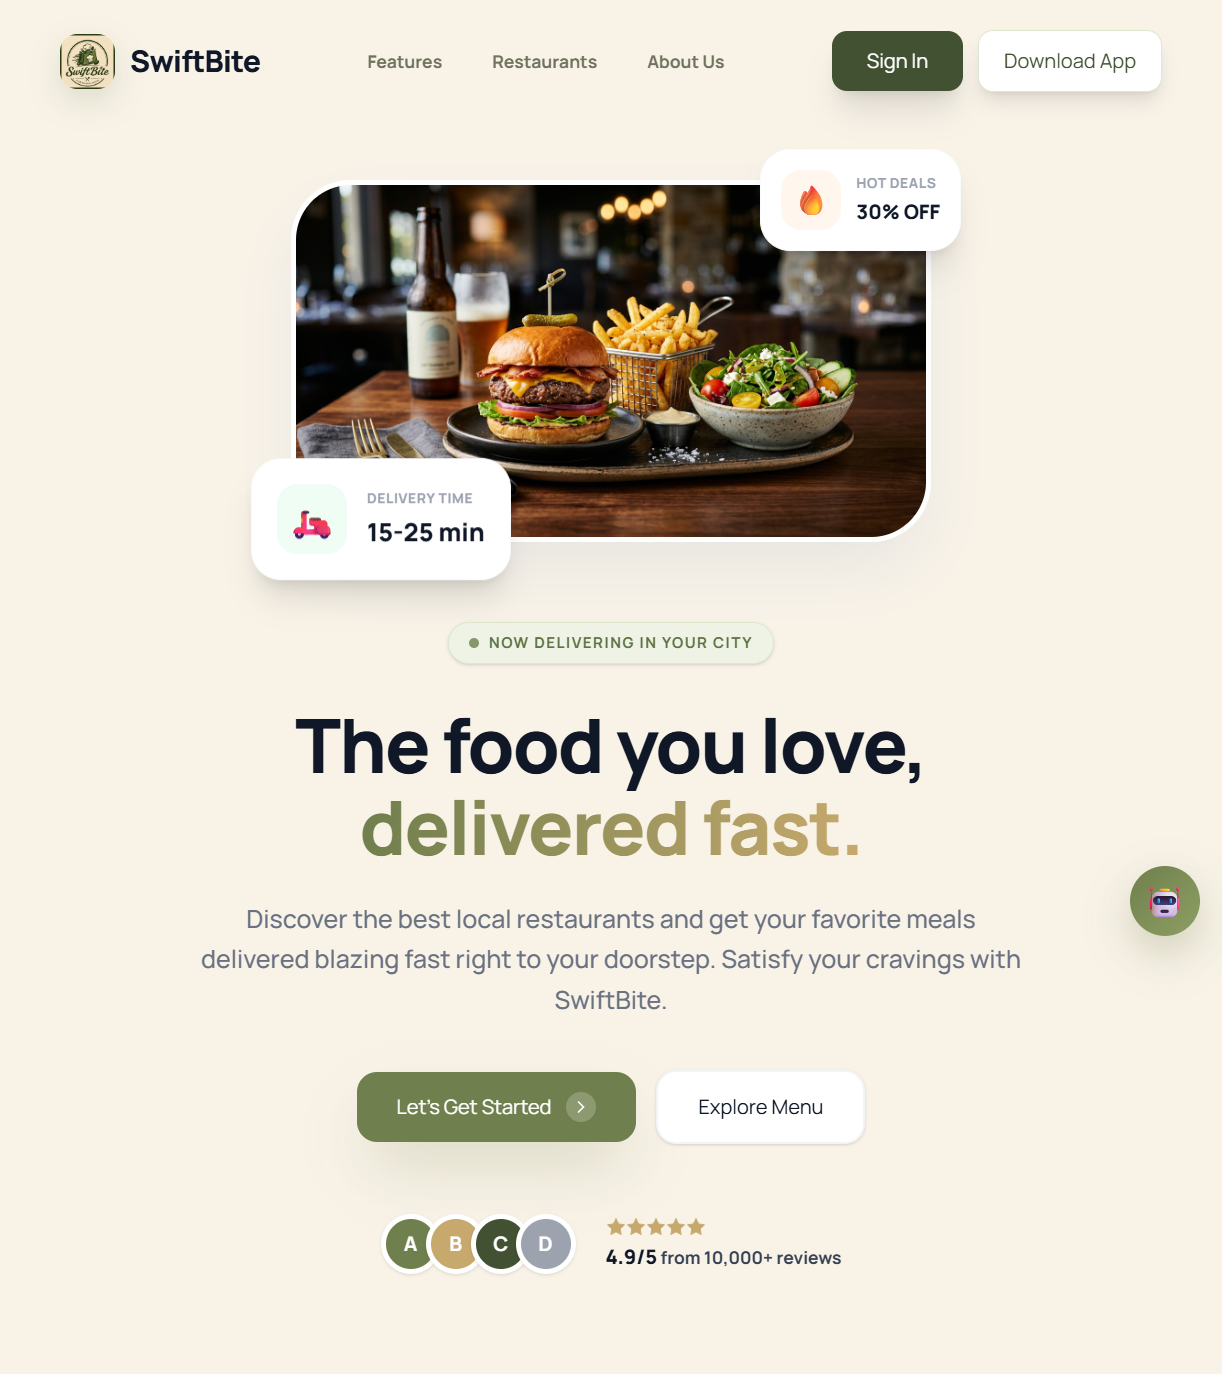
\includegraphics[width=0.9\textwidth,height=0.5\textheight,keepaspectratio]{Chapters/landing_page.png}
    \caption{Current SwiftBite landing page}
    \label{fig:landing_page}
\end{figure}

\begin{figure}[H]
    \centering
    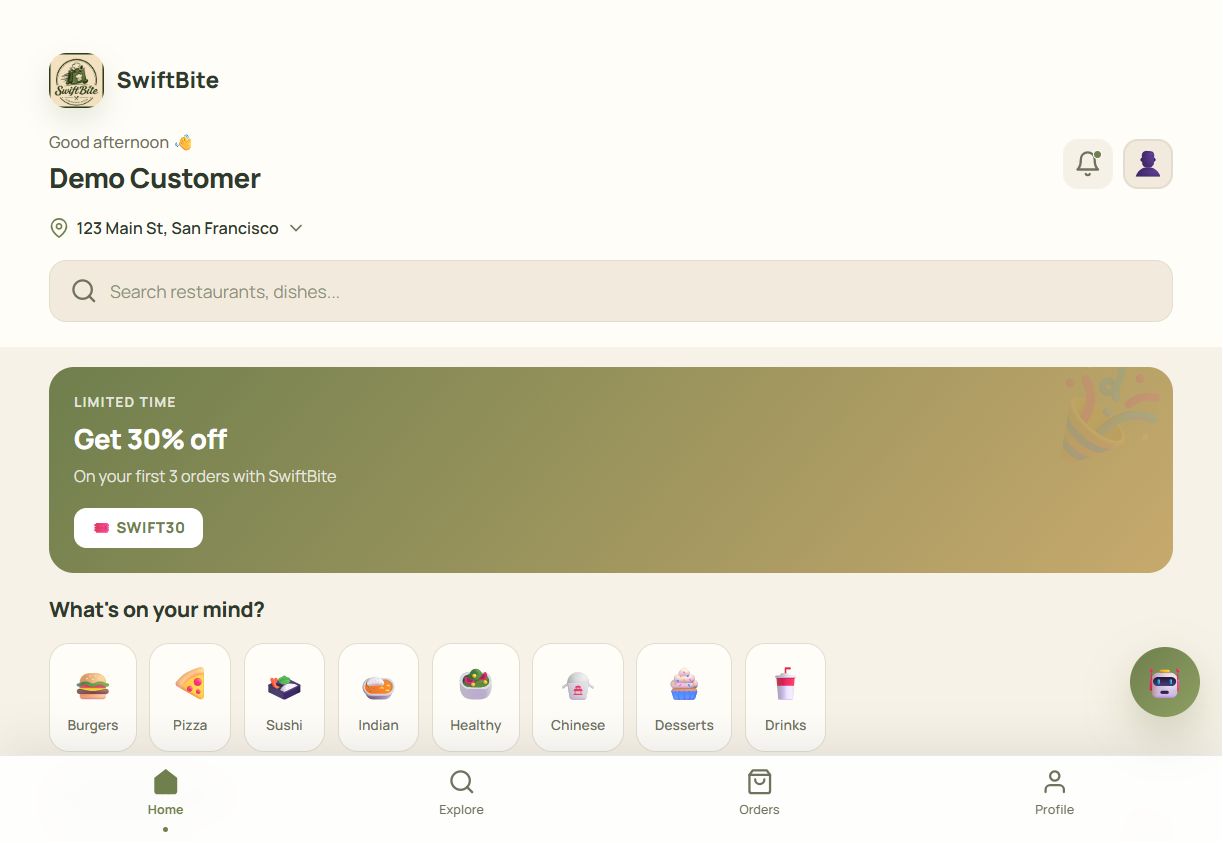
\includegraphics[width=0.9\textwidth,height=0.35\textheight,keepaspectratio]{Chapters/customer_home.png}
    \caption{Customer home screen showing the current promotion and food categories}
    \label{fig:customer_home}
\end{figure}

\subsection{Registration and Password Confirmation}

\begin{figure}[H]
    \centering
    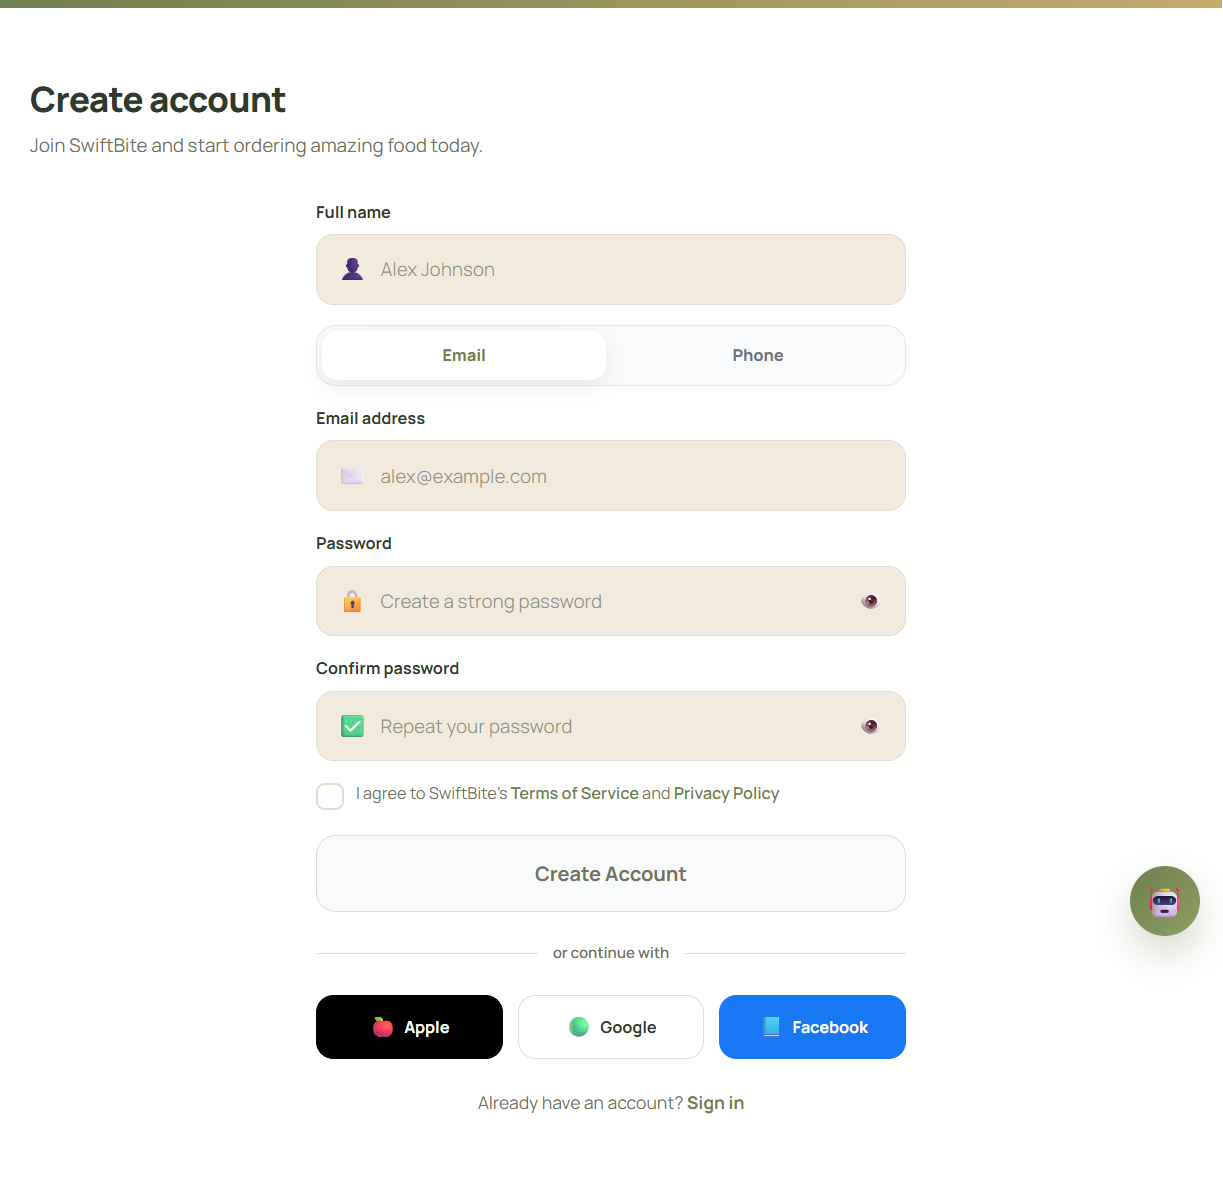
\includegraphics[width=0.72\textwidth,height=0.4\textheight,keepaspectratio]{Chapters/register.png}
    \caption{Current sign-up form, including the required confirm-password field}
    \label{fig:register_current}
\end{figure}

\begin{figure}[H]
    \centering
    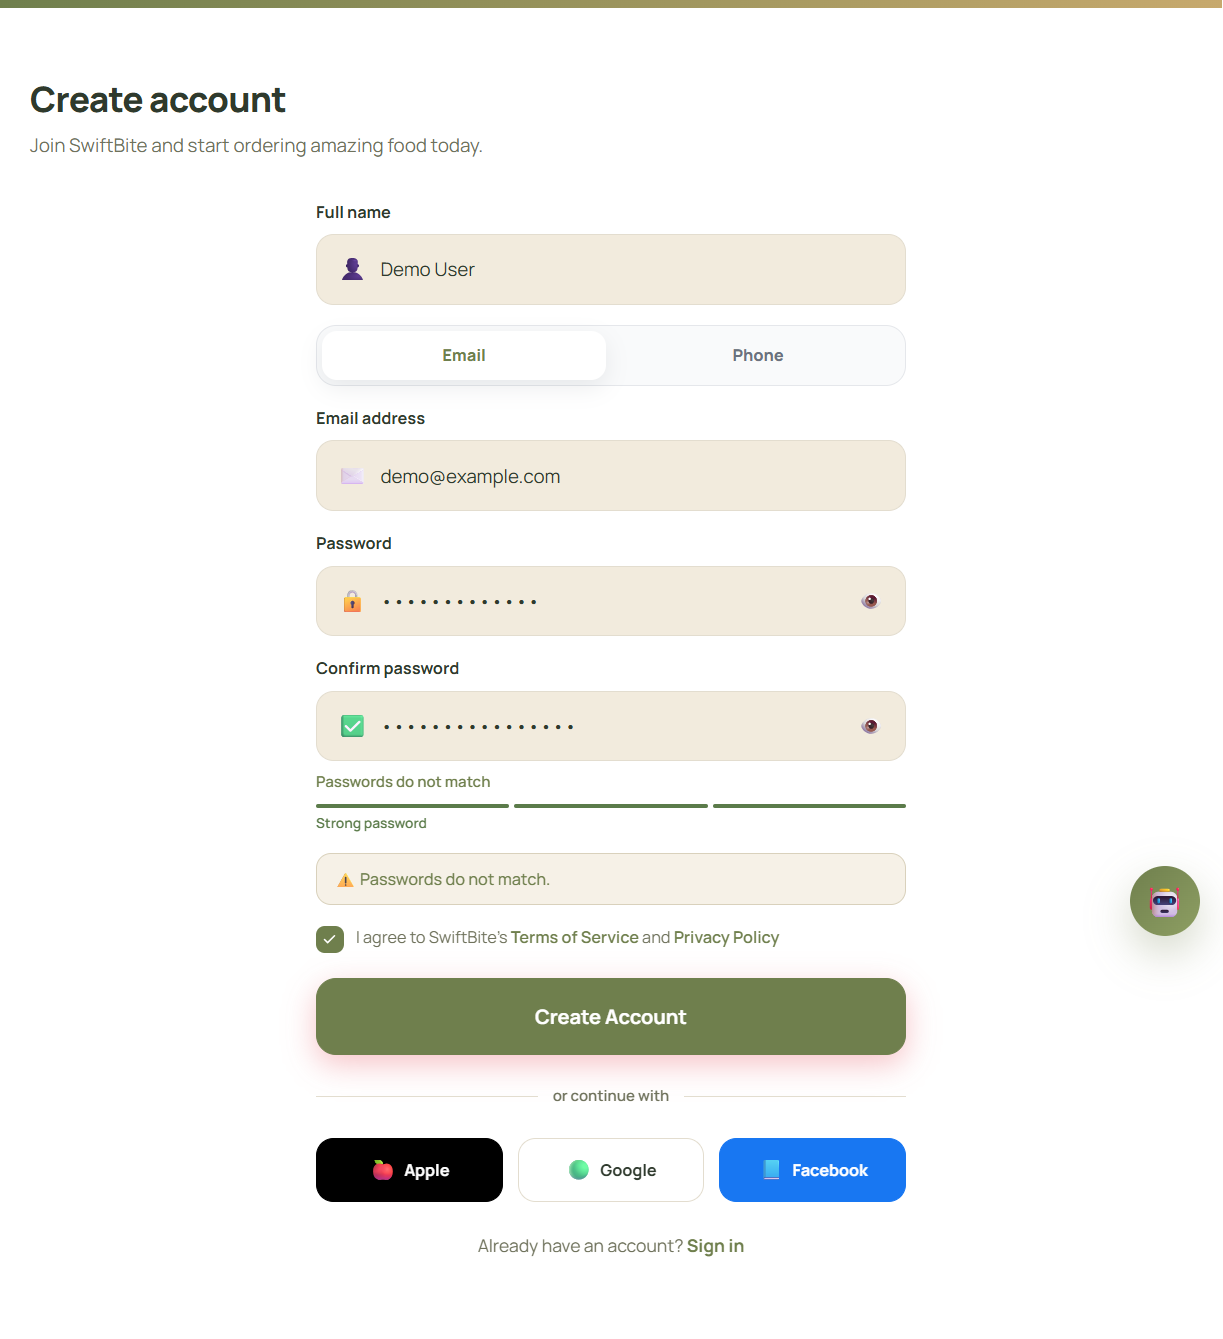
\includegraphics[width=0.72\textwidth,height=0.4\textheight,keepaspectratio]{Chapters/validation_error.png}
    \caption{Current sign-up validation when the password fields do not match}
    \label{fig:password_validation}
\end{figure}

\subsection{Restaurant Menu and Checkout}

\begin{figure}[H]
    \centering
    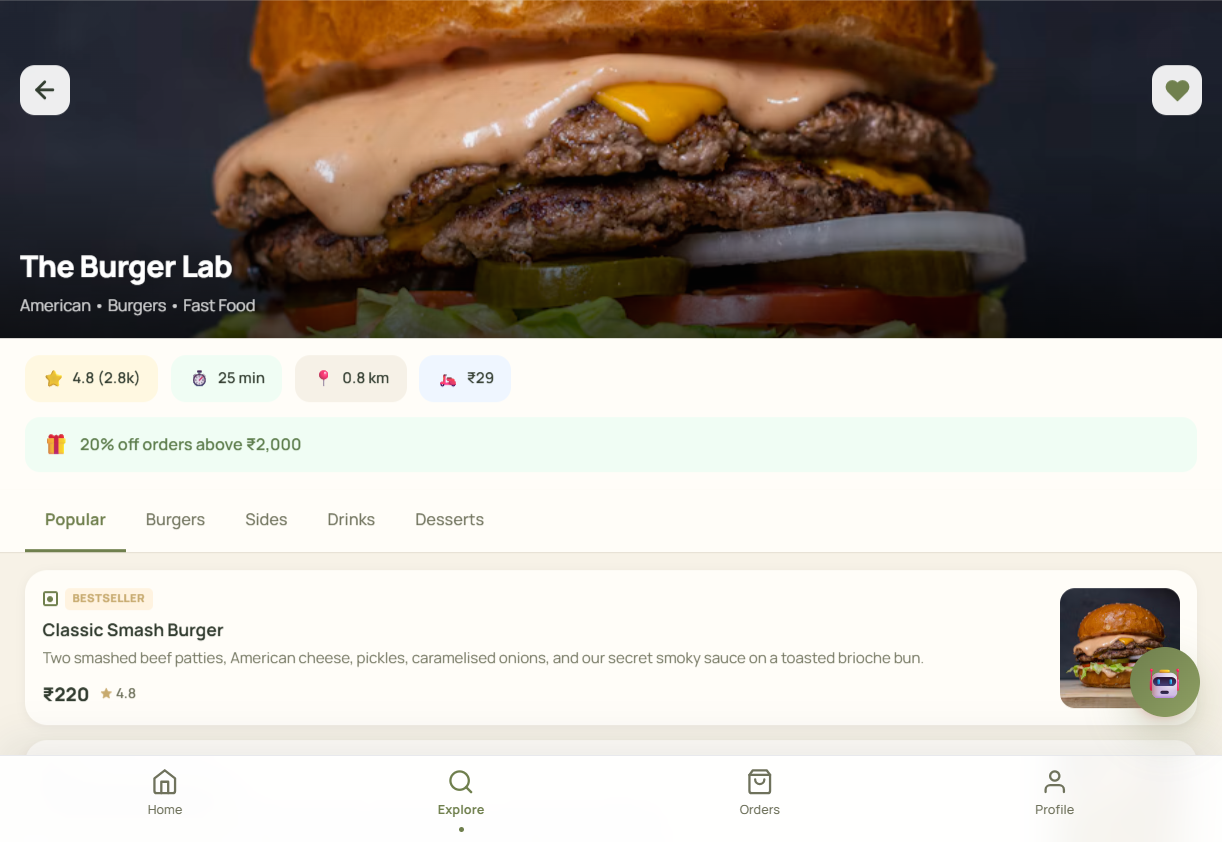
\includegraphics[width=0.9\textwidth,height=0.58\textheight,keepaspectratio]{Chapters/menu_list.png}
    \caption{Restaurant detail and sample menu}
    \label{fig:menu_current}
\end{figure}

\begin{figure}[H]
    \centering
    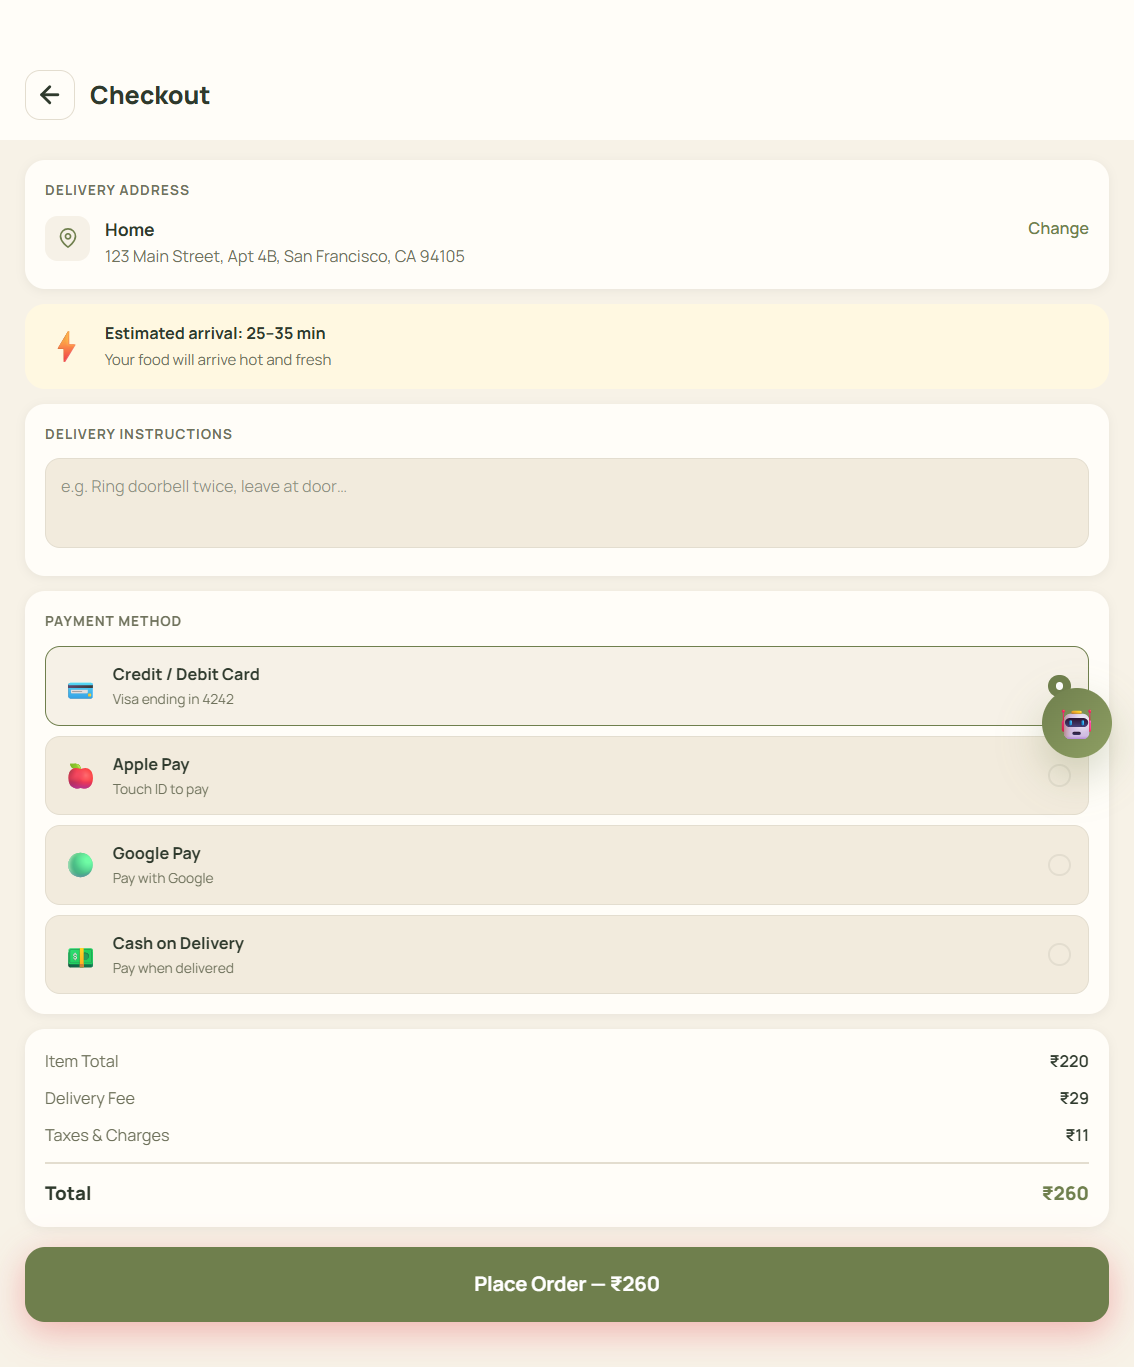
\includegraphics[width=0.9\textwidth,height=0.45\textheight,keepaspectratio]{Chapters/checkout.png}
    \caption{Checkout demonstration with delivery and payment-selection options}
    \label{fig:checkout_current}
\end{figure}

\subsection{Order Status, Chatbot, and Portal Switching}

\begin{figure}[H]
    \centering
    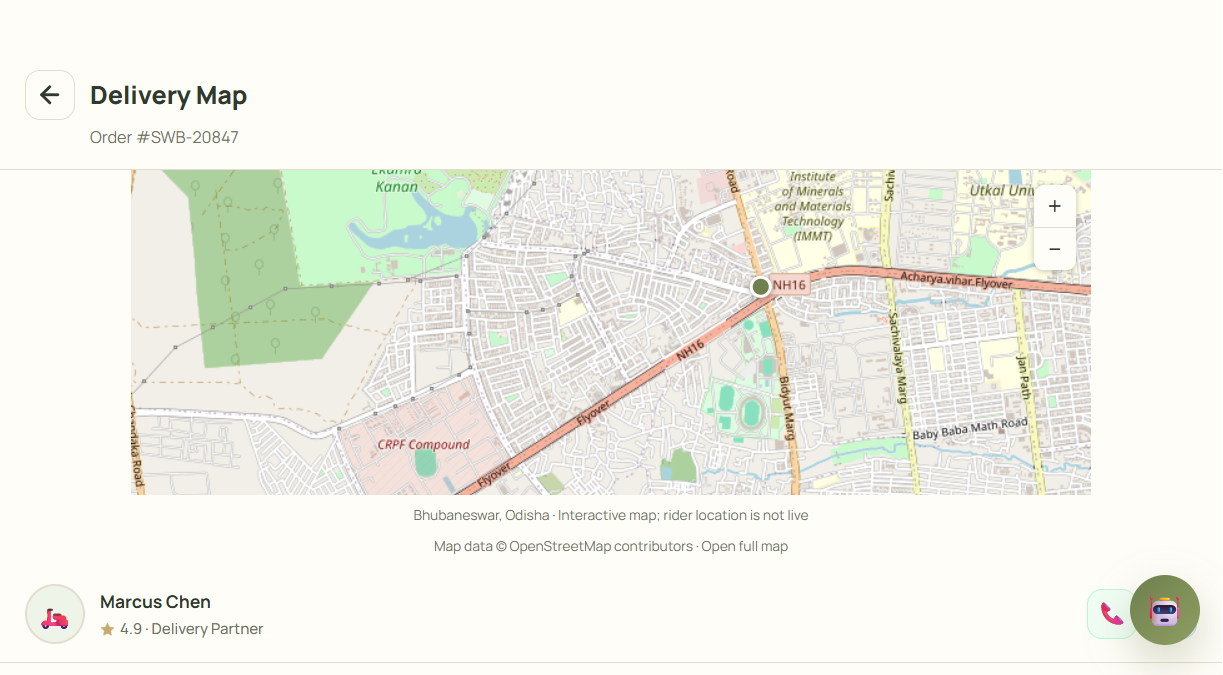
\includegraphics[width=0.9\textwidth,height=0.9\textheight,keepaspectratio]{Chapters/order_tracking_bhubaneswar_app.png}
    \caption{SwiftBite delivery screen with zoomable OpenStreetMap tiles centered on Bhubaneswar; rider location is not live}
    \label{fig:tracking_current}
\end{figure}

\begin{figure}[H]
    \centering
    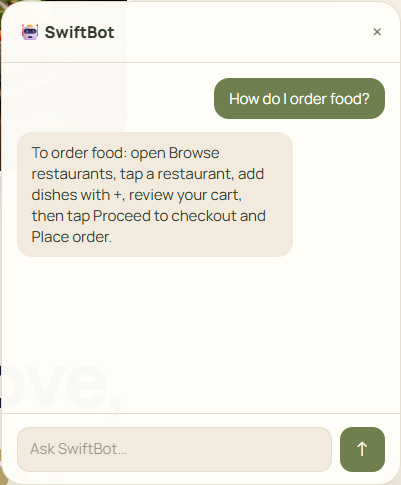
\includegraphics[width=0.9\textwidth,height=0.4\textheight,keepaspectratio]{Chapters/chatbot_test.png}
    \caption{Local rule-based chatbot fallback response to an app-guidance question}
    \label{fig:chatbot_current}
\end{figure}

\begin{figure}[H]
    \centering
    \vspace*{2cm}
    \hspace*{3.5cm}
    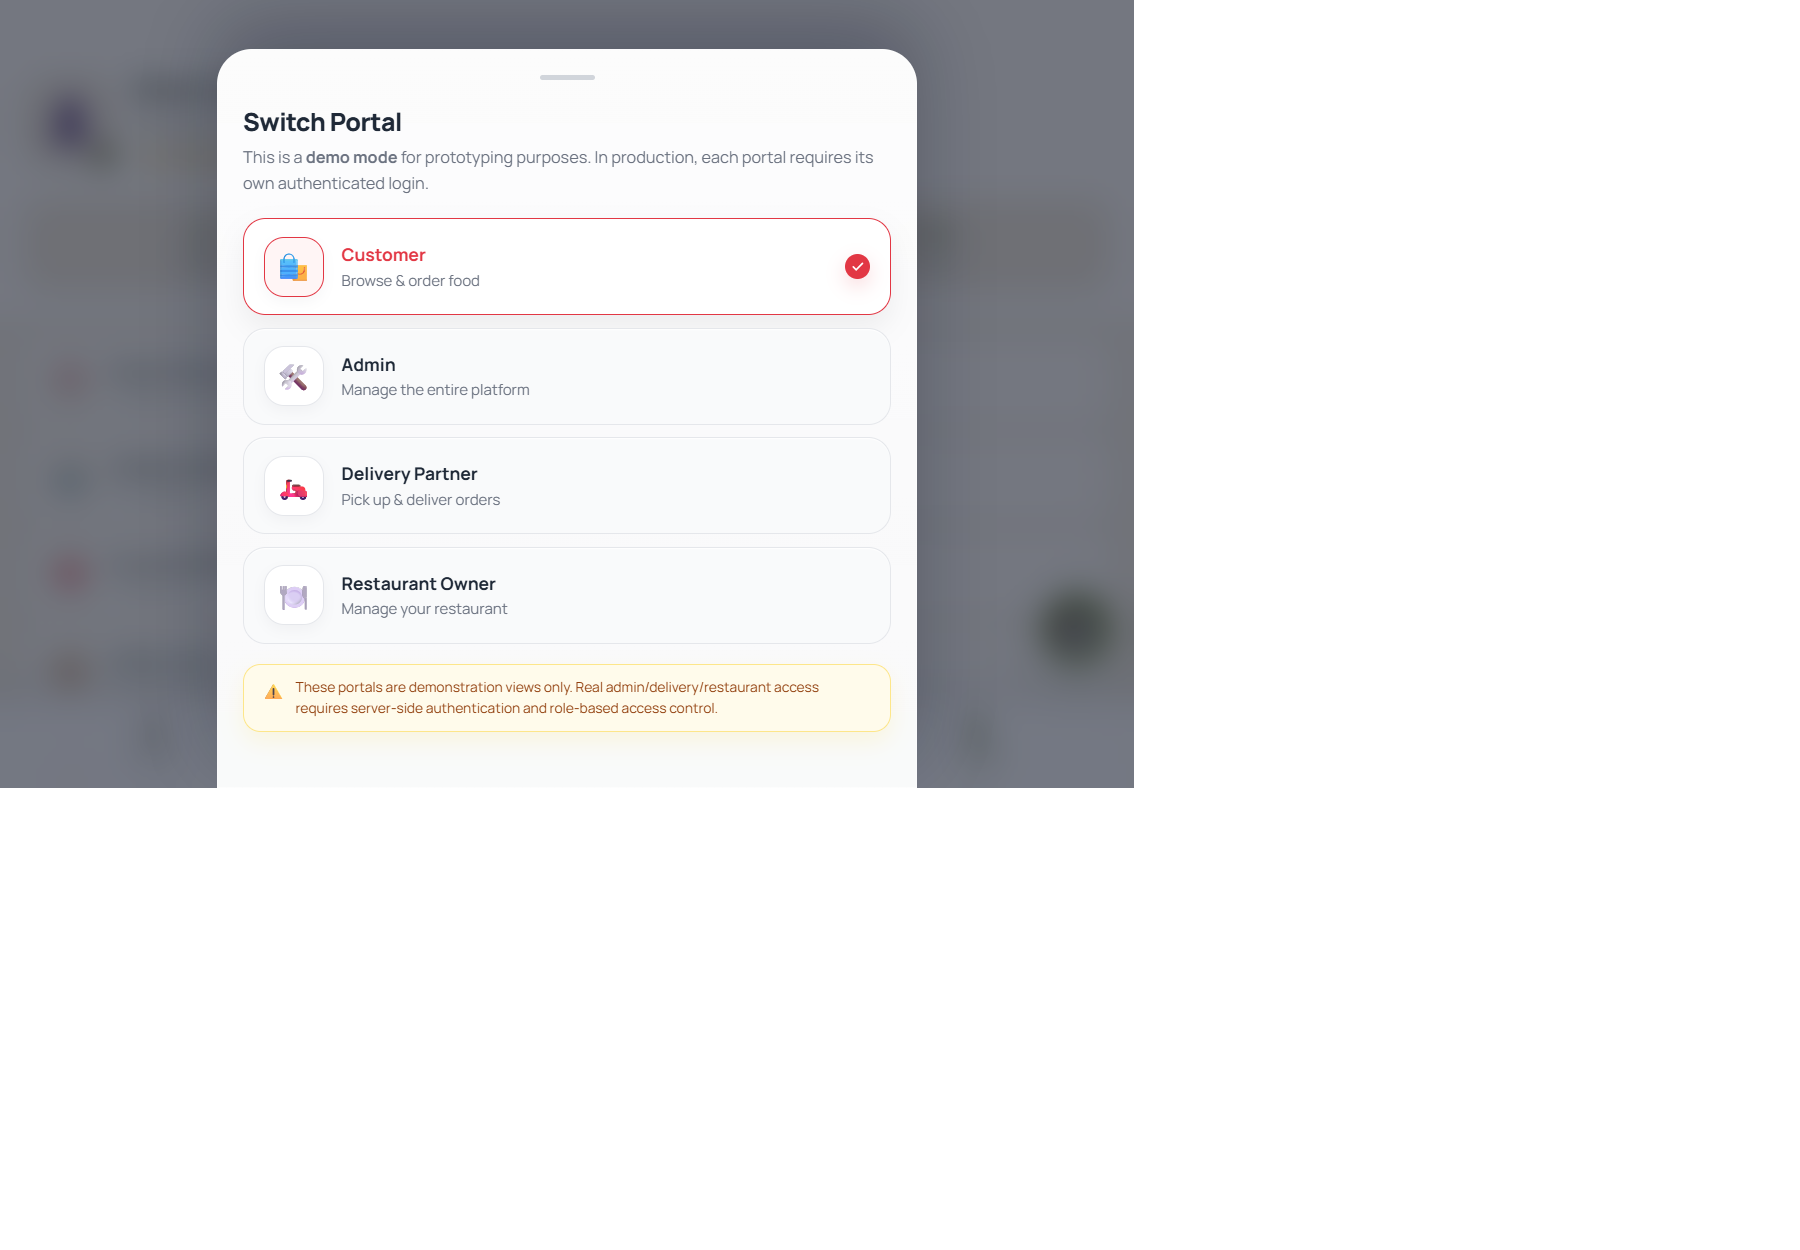
\includegraphics[
        width=0.9\textwidth,
        height=0.4\textheight,
        keepaspectratio
    ]{Chapters/role_selection.png}

    \caption{Portal switcher, explicitly identified in the application as demo functionality}
    \label{fig:portal_switcher}
\end{figure}

\chapter{Software Testing}

Testing for SwiftBite covered the frontend and backend builds, registration validation, visible prototype workflows, and the working MySQL integration. A read-only query succeeded, the schema was initialized, and the restaurant API was confirmed to return MySQL-backed records. Full authentication and order-persistence integration tests were not performed.

\section{Test Plan and Objectives}

The verification plan covered:
\begin{itemize}
    \item Compilation of the frontend and backend TypeScript projects.
    \item Direct MySQL connectivity, schema initialization, and the database-backed restaurant API response.
    \item Presence and use of the sign-up confirm-password field.
    \item Client-side handling of empty and mismatched registration values.
    \item Rendering of the customer home, menu, checkout, order-status, chatbot, and portal-switcher screens.
    \item Clear identification of the checkout, order, and portal flows as demonstrations rather than live production integrations.
\end{itemize}

\section{Testing Methodologies}

\subsection{Build and Type Checking}
The frontend production build, frontend TypeScript check, and backend TypeScript build were run to identify compilation and type errors.

\subsection{Manual Browser Verification}
The current frontend was opened in a browser. The sign-up screen was checked with mismatched password values, and the resulting validation message was confirmed. Screenshots in this report were captured from the current frontend. These checks do not substitute for automated end-to-end testing against a configured production API.

\subsection{MySQL and API Verification}
A read-only \texttt{SELECT 1} query succeeded against MySQL. The eight-table schema was initialized with four restaurants and four categories. \texttt{GET /api/restaurants} returned four records with the response source identified as MySQL. Registration, login, and persistent order creation were not exercised in this verification.

\section{Test Cases and Results}

\begin{table}[H]
\centering
\caption{Verification Cases}
\label{tab:test_cases}
\renewcommand{\arraystretch}{1.35}
\begin{tabular}{|l|p{3.4cm}|p{6.5cm}|l|}
\hline
\textbf{ID} & \textbf{Feature} & \textbf{Verification} & \textbf{Result} \\
\hline
TC\_01 & Frontend build & Run \texttt{npm run build} in the frontend project. & PASS \\
\hline
TC\_02 & Frontend types & Run \texttt{npx tsc --noEmit} in the frontend project. & PASS \\
\hline
TC\_03 & Backend types & Run \texttt{npm run build} in the backend project. & PASS \\
\hline
TC\_04 & Password confirmation & Enter two different password values in sign-up and submit; the UI displays a mismatch error and does not send the registration request. & PASS \\
\hline
TC\_05 & Prototype screens & Open the current home, restaurant menu, checkout, tracking, chatbot, and portal-switcher interfaces. & PASS \\
\hline
TC\_06 & MySQL connection and schema & Run a read-only query, initialize the schema, and confirm the restaurant API returns database-backed records. & PASS \\
\hline
TC\_07 & Auth/order integration & Exercise registration, login, and persistent order flows against the backend and MySQL instance. & NOT RUN \\
\hline
\end{tabular}
\end{table}
\newpage
\subsection{Password Confirmation Validation}
\textbf{Objective:} Confirm that the registration form does not proceed when the two password fields differ. \\
\textbf{Result:} The browser displayed both the inline mismatch message and the form error; the registration request was not submitted. Figure \ref{fig:password_validation} shows this validation state.

\begin{figure}[H]
    \centering
    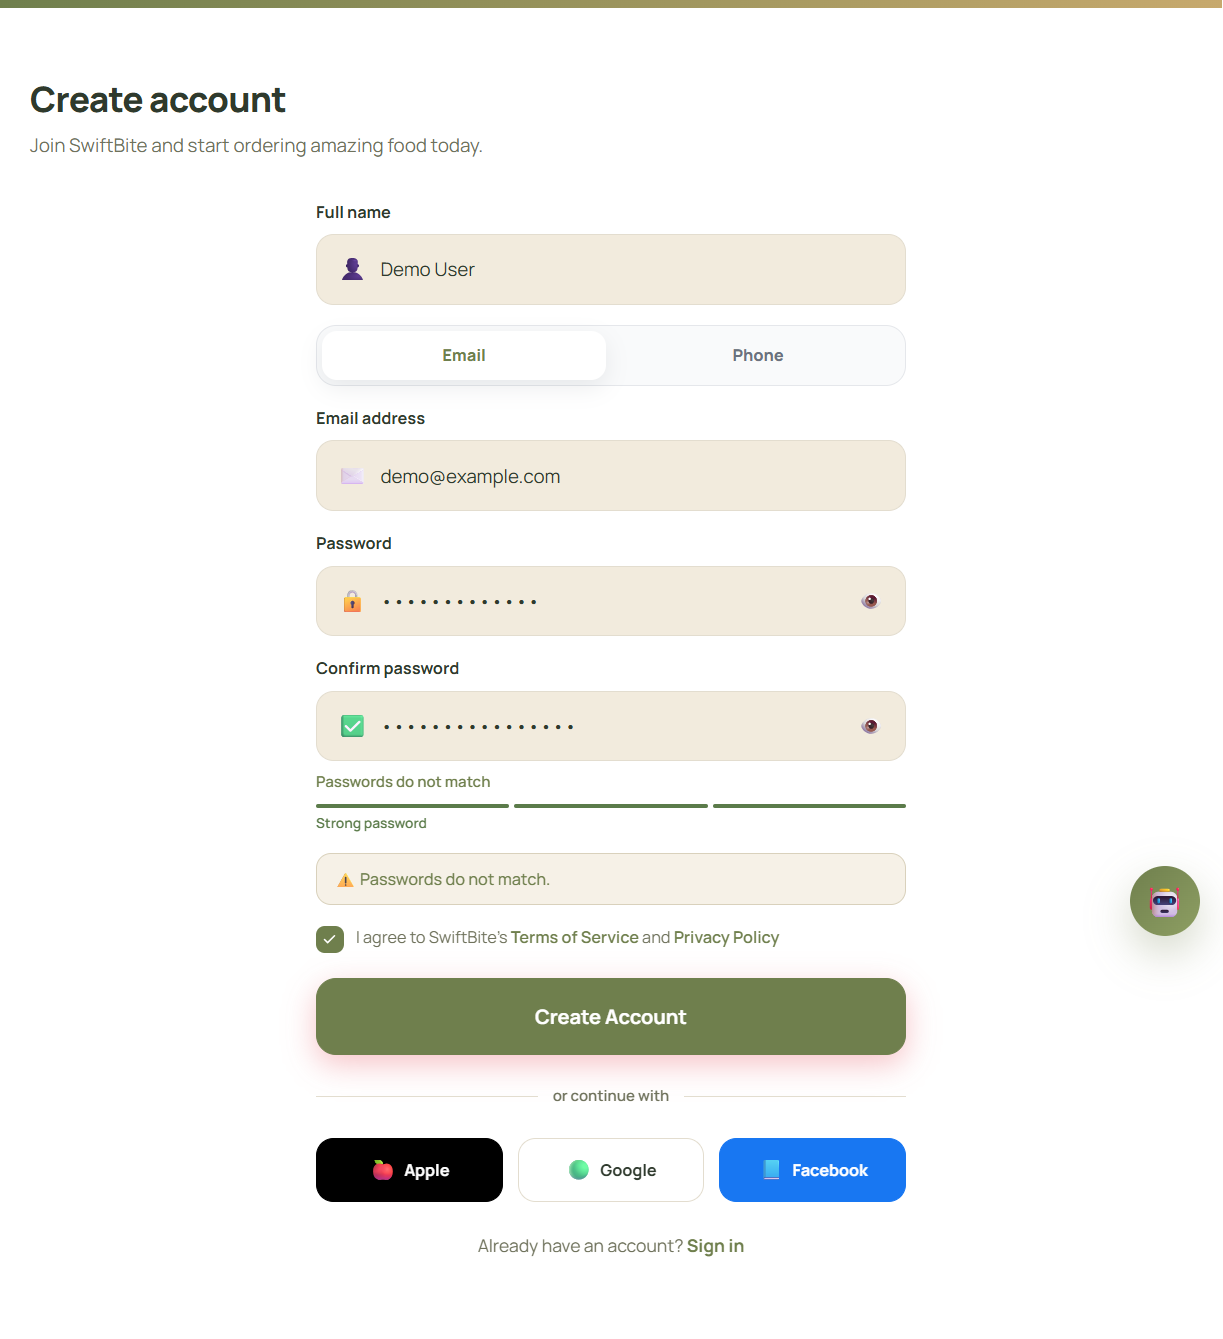
\includegraphics[width=0.72\textwidth,height=0.62\textheight,keepaspectratio]{Chapters/validation_error.png}
    \caption{Sign-up form rejecting mismatched passwords}
    \label{fig:test_validation}
\end{figure}

\subsection{Registration Form}
\textbf{Objective:} Verify the current sign-up fields and required confirmation entry. \\
\textbf{Result:} The current screen presents name, email or phone selection, password, confirm password, and terms acceptance. Successful registration against a live backend was not verified in this browser session.

\begin{figure}[H]
    \centering
    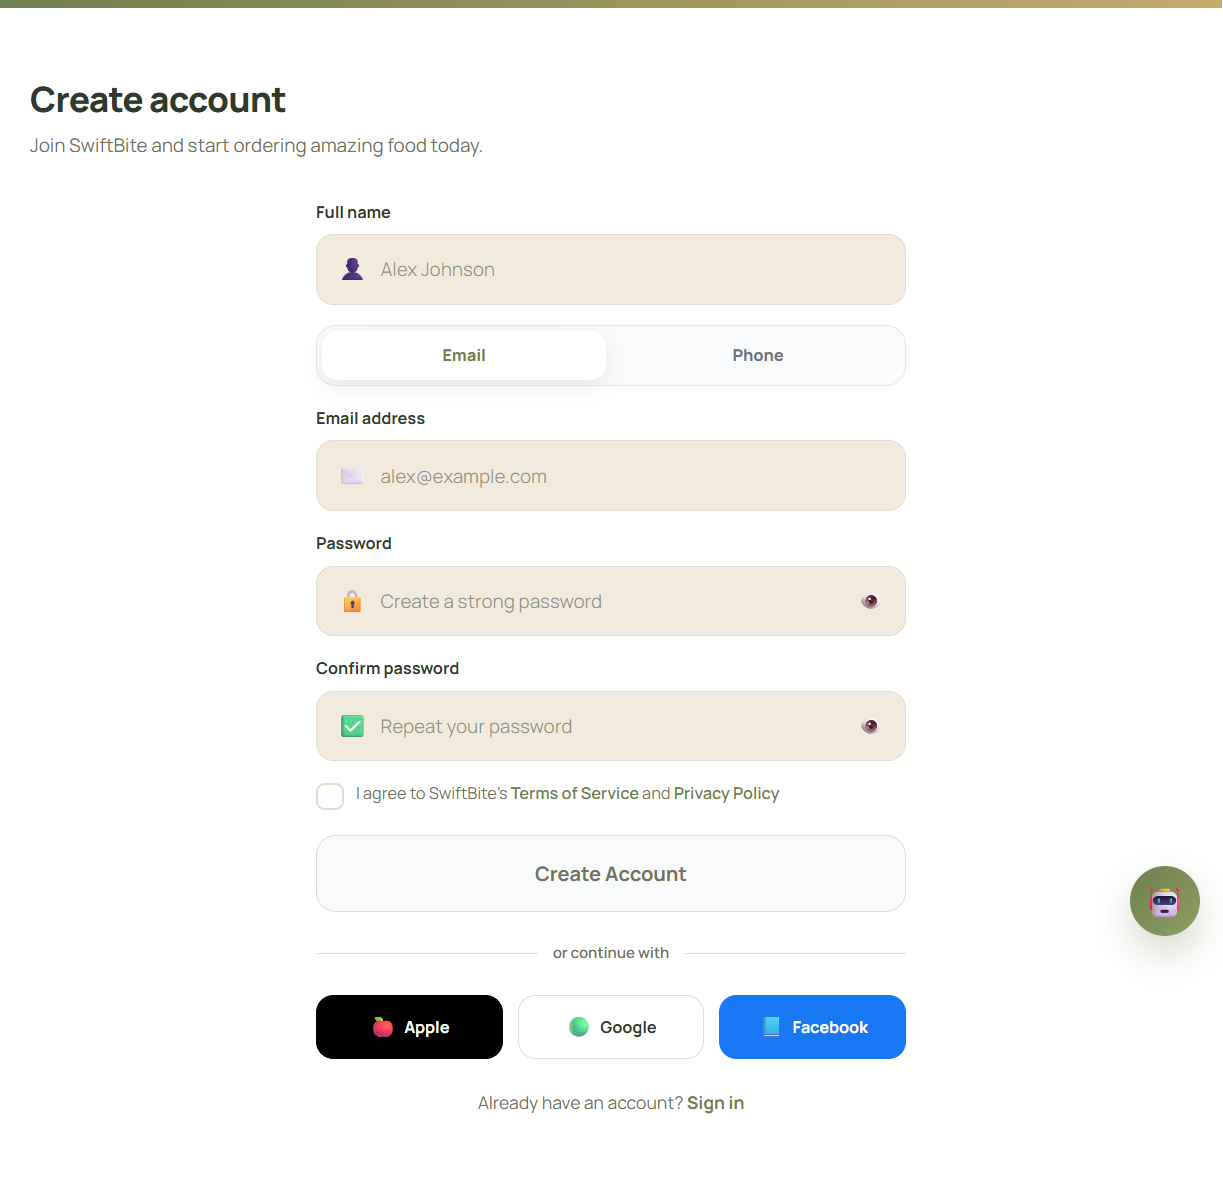
\includegraphics[width=0.72\textwidth,height=0.62\textheight,keepaspectratio]{Chapters/register.png}
    \caption{Current SwiftBite sign-up form}
    \label{fig:test_register}
\end{figure}

\subsection{Scope of Verification}
The customer menu, checkout, order-status, and portal-switcher interfaces render in the browser. The MySQL connection, schema, and restaurant-list API were verified, but the customer catalogue still uses bundled sample data. Checkout does not persist orders or charge a payment method, and the tracking screen does not use GPS. Registration, login, and order-writing routes require separate integration tests.

\section{Testing Conclusion}

The frontend and backend builds and TypeScript checks completed successfully, the sign-up password-mismatch validation was confirmed in the browser, and MySQL connectivity and the restaurant API were verified. These checks do not establish persistent customer ordering, payment processing, GPS tracking, or production authentication behavior.

\chapter{Results and Discussion}
\vspace{-1cm}
\section{Overview}

The current SwiftBite result is an interactive web prototype with a React-based customer experience and a separate Express API. The frontend demonstrates the principal screens of a food-ordering journey, while several operational integrations remain incomplete. This chapter presents current application screenshots and discusses what the implementation does and does not demonstrate.

\section{Current Application Outputs}
\vspace{-0.5cm}
\subsection{Landing Page and Customer Home}

The landing page introduces the SwiftBite service. The home screen includes restaurant cards, categories, offers, and popular dishes; the screenshot shows the promotion and food categories at the top of the page. Restaurant and menu content is bundled in frontend sample data rather than dynamically loaded from MySQL in the current customer flow.

\begin{figure}[H]
    \centering
    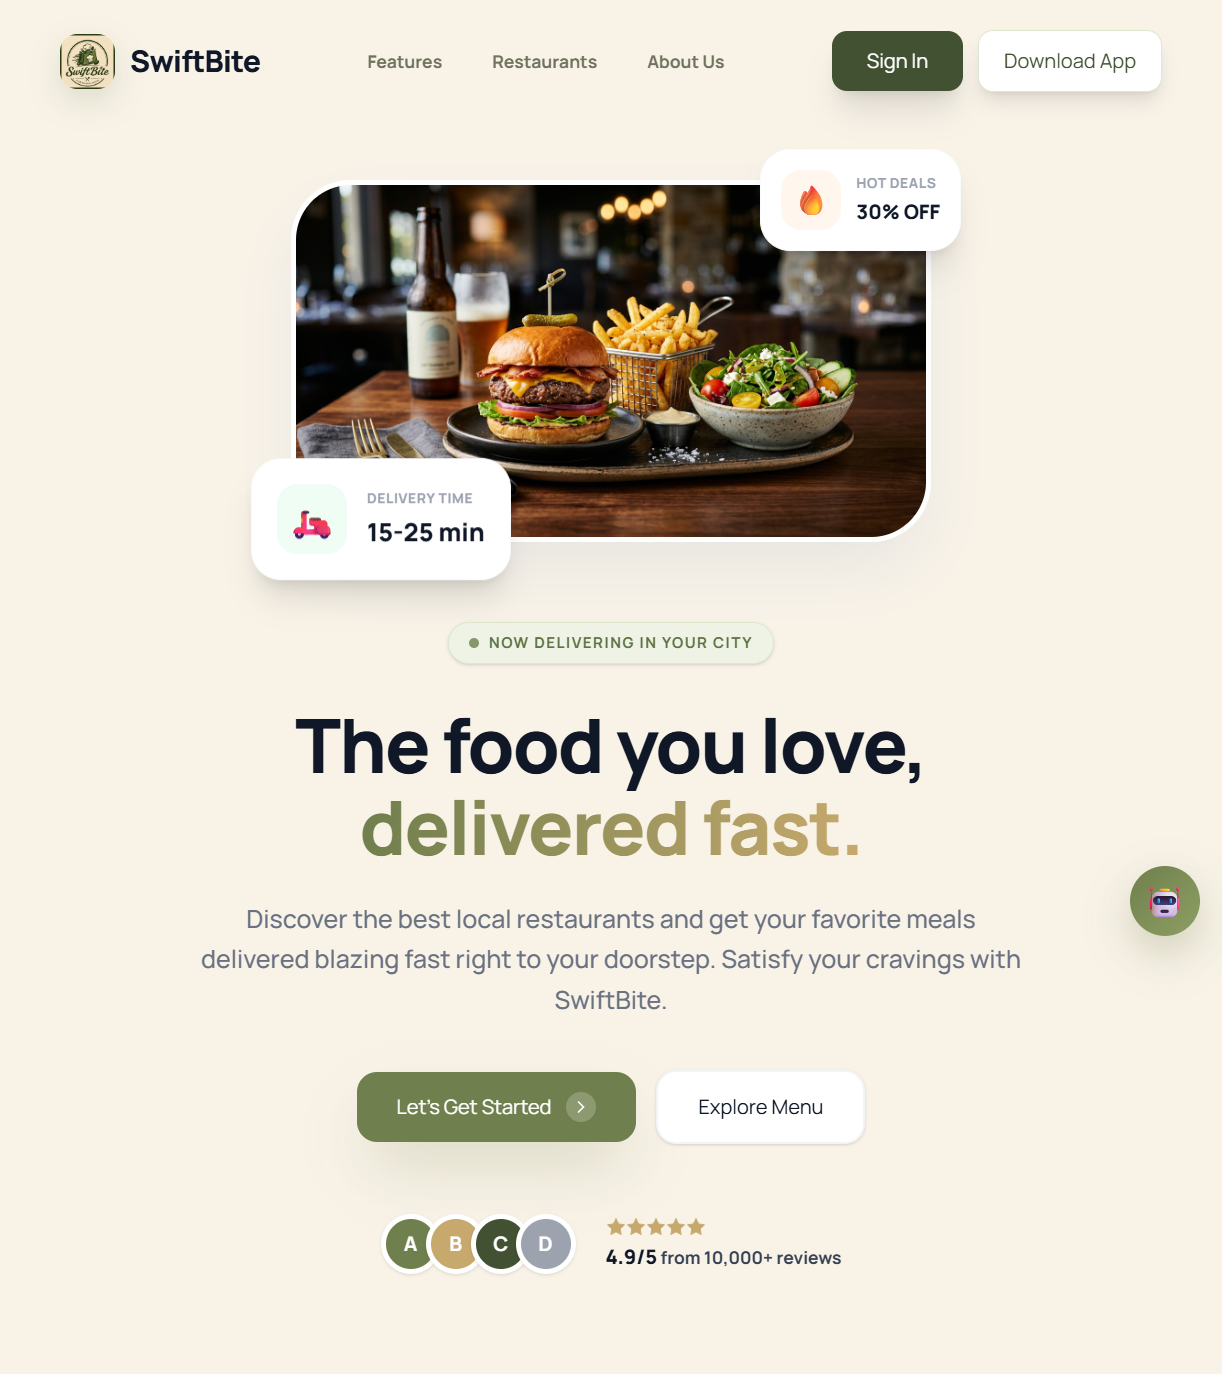
\includegraphics[width=0.9\textwidth,height=0.5\textheight,keepaspectratio]{Chapters/landing_page.png}
    \caption{Current SwiftBite landing page}
    \label{fig:result_landing}
\end{figure}

\begin{figure}[H]
    \centering
    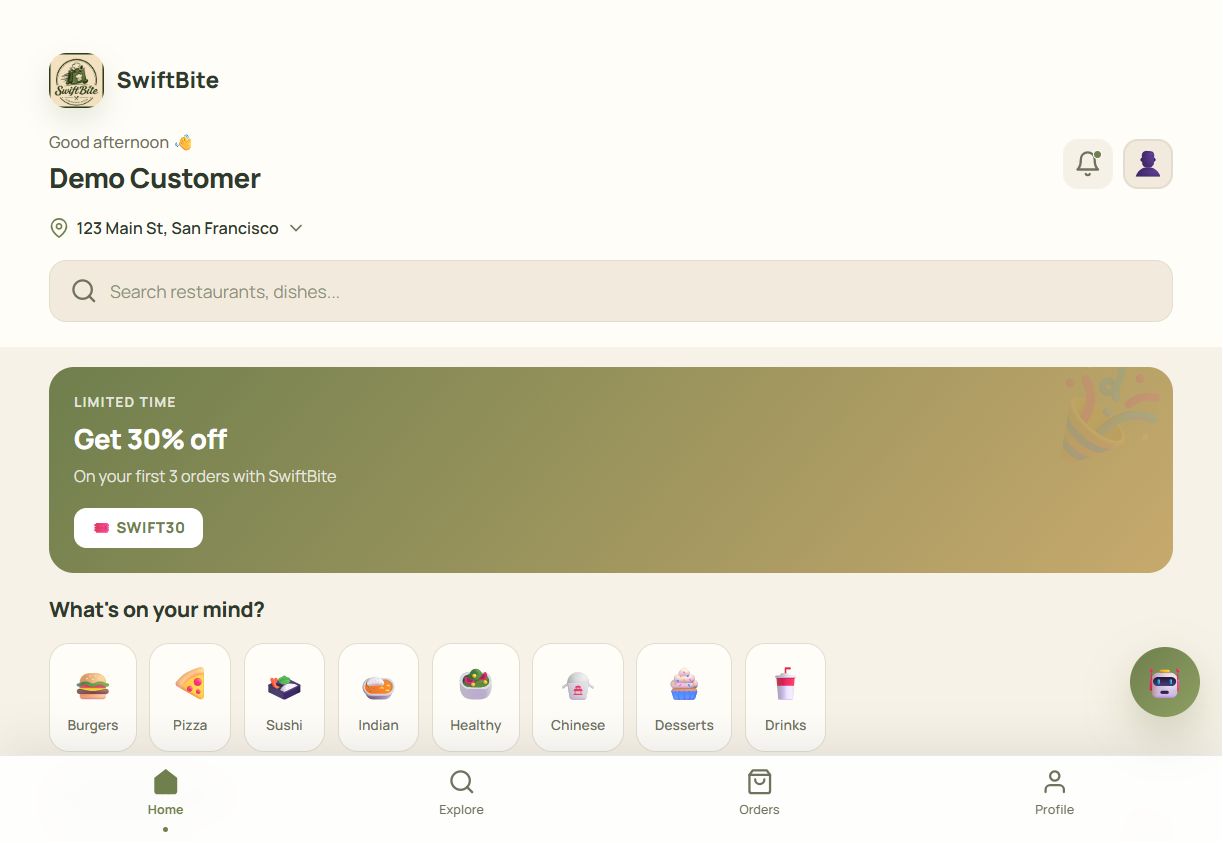
\includegraphics[width=0.9\textwidth,height=0.4\textheight,keepaspectratio]{Chapters/customer_home.png}
    \caption{Customer home screen showing the promotion and food categories}
    \label{fig:result_home}
\end{figure}

\subsection{Restaurant and Menu Browsing}

The restaurant detail screen displays a sample restaurant, category controls, menu items, and cart quantity actions. These interactions demonstrate the frontend workflow and use local state.

\begin{figure}[H]
    \centering
    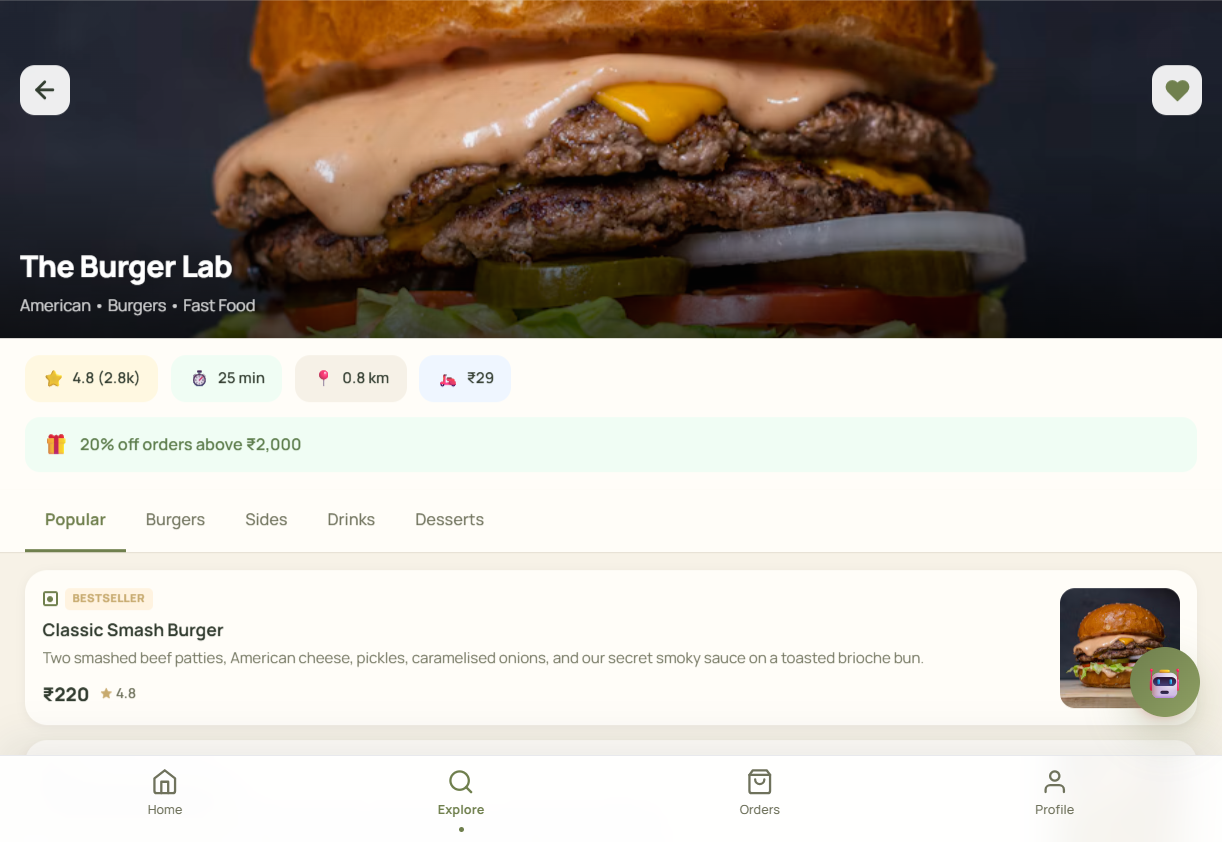
\includegraphics[width=0.9\textwidth,height=0.3\textheight,keepaspectratio]{Chapters/menu_list.png}
    \caption{Restaurant details and sample menu items}
    \label{fig:result_menu}
\end{figure}

\subsection{Account Registration}

The sign-up form accepts an email address or phone number and includes required password confirmation. The frontend checks that the password fields match before submitting; the backend registration schema also requires a matching confirmation value.

\begin{figure}[H]
    \centering
    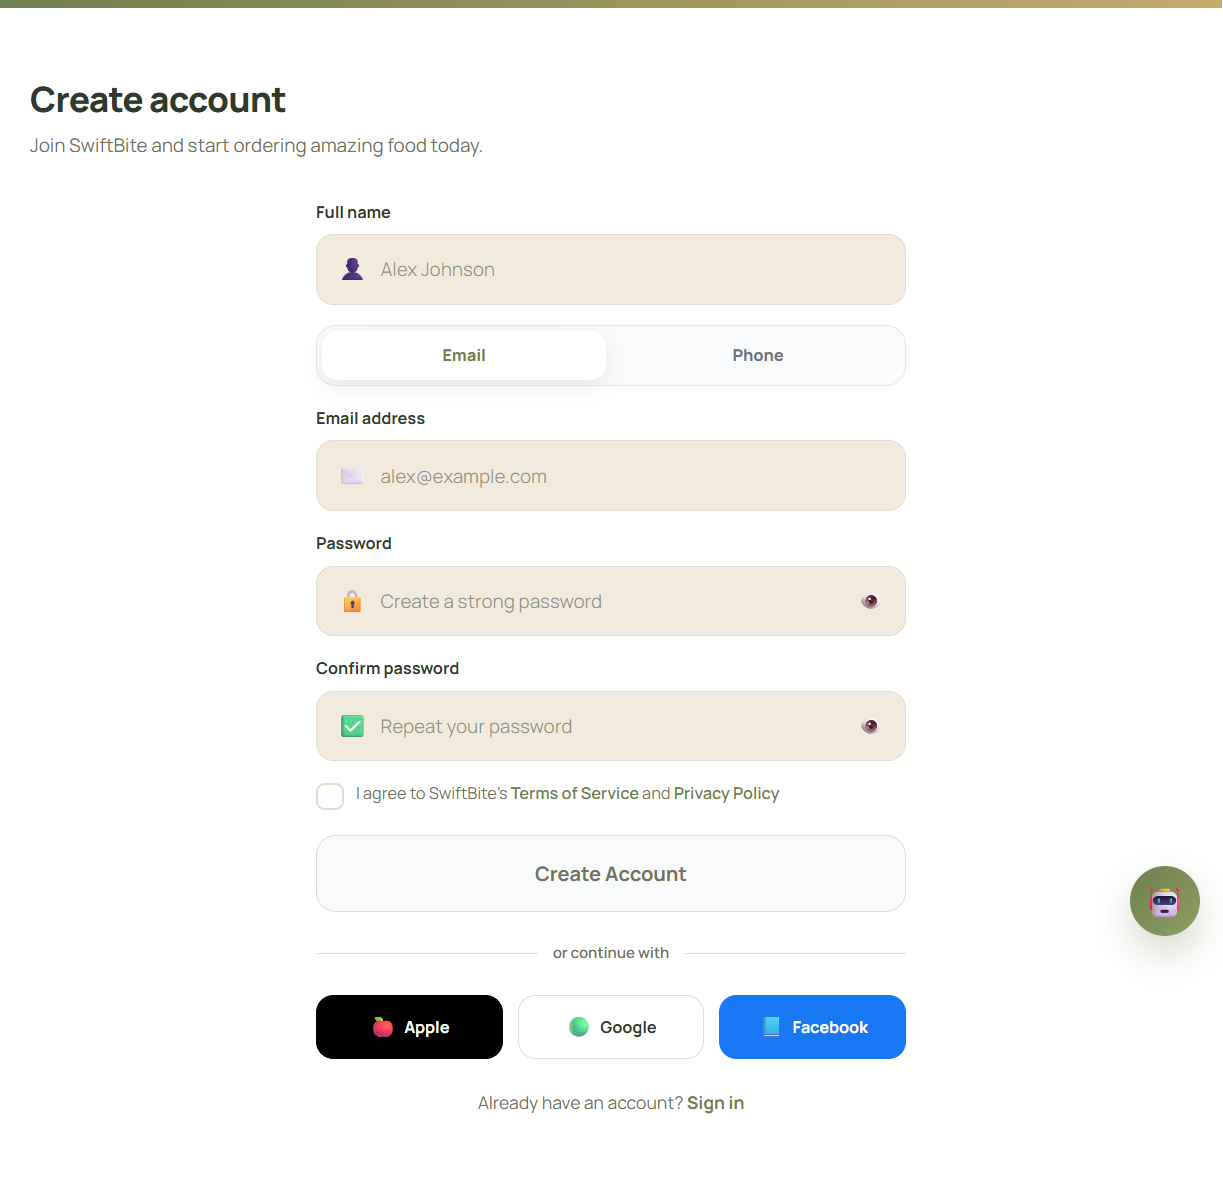
\includegraphics[width=0.72\textwidth,height=0.3\textheight,keepaspectratio]{Chapters/register.png}
    \caption{Current sign-up form with password confirmation}
    \label{fig:result_register}
\end{figure}

\subsection{Checkout and Order-Status Demonstrations}

The cart and checkout screens show quantity totals, delivery details, and payment choices. In the current frontend, selecting Place Order advances to a demonstration confirmation and order-status flow. It does not create a persistent order, process a payment, or retrieve live delivery coordinates.

\begin{figure}[H]
    \centering
    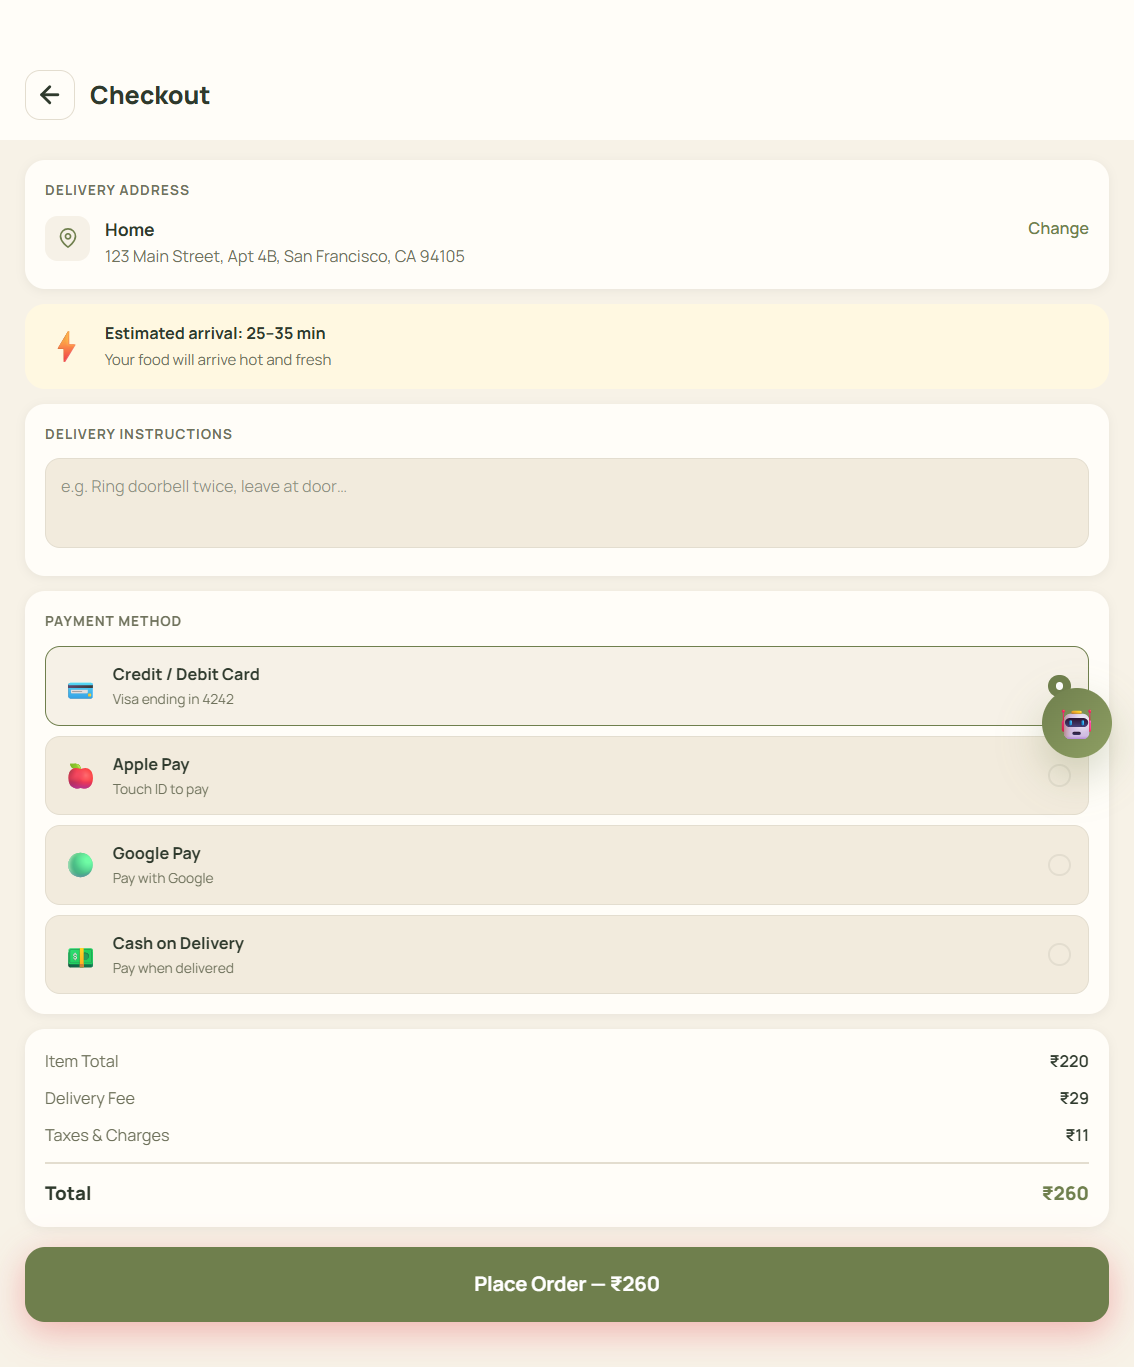
\includegraphics[width=0.9\textwidth,height=0.4\textheight,keepaspectratio]{Chapters/checkout.png}
    \caption{Checkout screen demonstrating delivery and payment selection}
    \label{fig:result_checkout}
\end{figure}

\begin{figure}[H]
    \centering
    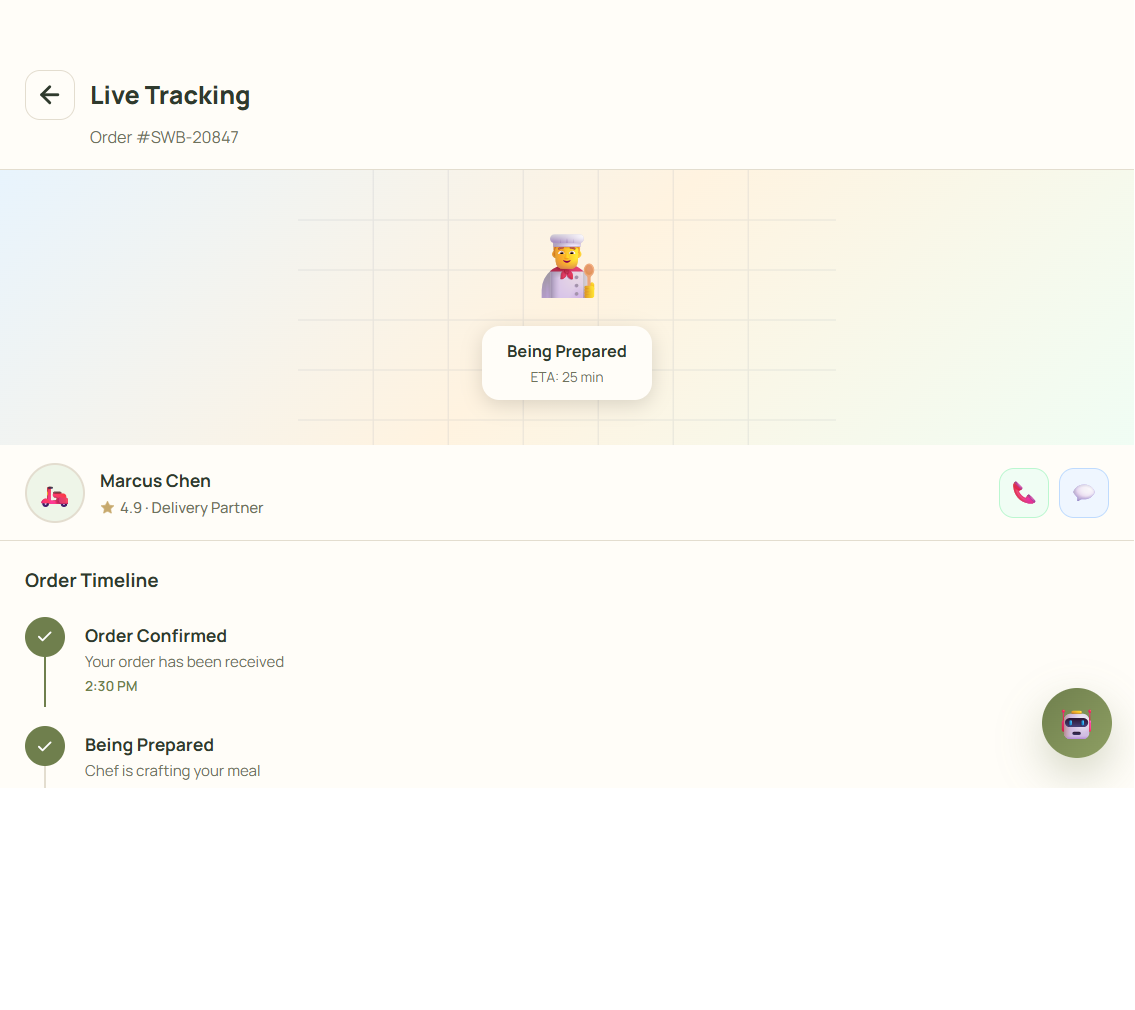
\includegraphics[width=0.9\textwidth,height=0.35\textheight,keepaspectratio]{Chapters/order_tracking.png}
    \caption{Demonstration order-status screen; not live GPS tracking}
    \label{fig:result_tracking}
\end{figure}

\subsection{Chatbot Assistance}

The chatbot responds to application questions. The frontend can use local rule-based responses when no API base URL is configured; the backend can call Gemini when its server-side key is present. The chatbot is an assistance feature and does not provide personalized food recommendations or place orders.

\begin{figure}[H]
    \centering
    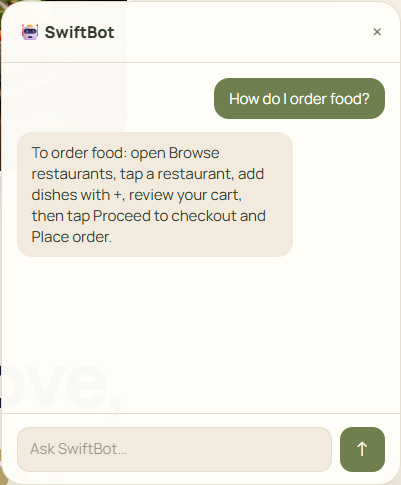
\includegraphics[width=0.9\textwidth,height=0.58\textheight,keepaspectratio]{Chapters/chatbot_test.png}
    \caption{Chatbot answering a food-ordering navigation question}
    \label{fig:result_chatbot}
\end{figure}

\section{Discussion of Findings}

\begin{itemize}
    \item \textbf{Frontend implementation:} React, TypeScript, and Vite provide a component-based interface. The customer catalogue and order journey currently use sample data and local state.
    \item \textbf{Backend capabilities:} The Express API includes authentication, profile, restaurant, menu, upload, order, dashboard, and chatbot routes. The storefront currently uses the authentication and chatbot services rather than integrating every available backend route.
    \item \textbf{Validation:} Zod validates backend request payloads. Registration requires password confirmation, and the frontend displays a mismatch error before sending the request.
    \item \textbf{Chatbot behavior:} Gemini is optional. Local rule-based responses allow app guidance without a configured model key or API base URL.
\end{itemize}

\section{Challenges and Current Constraints}

\begin{itemize}
    \item The frontend customer catalogue, cart, and checkout are not connected to persistent restaurant and order records.
    \item Payment methods are interface options only; there is no payment gateway or transaction processing.
    \item Order status is a demonstration screen and does not receive live events or GPS coordinates.
    \item Portal switching is demo functionality and does not enforce production server-side role authorization.
    \item The working MySQL connection, initialized schema, and database-backed restaurant API were verified. Full registration, login, and order-persistence integration tests remain outstanding; the file-backed authentication fallback is not a production persistence strategy.
\end{itemize}

\section{Summary}

SwiftBite currently demonstrates a responsive food-ordering interface, registration validation, a collection of backend API routes, and chatbot assistance. Its screenshots and results should be understood as prototype evidence. Persistent customer orders, real payment processing, live delivery tracking, and production-grade access control require further implementation and integration testing.

\chapter{Work Done So Far}

This chapter records the current implementation of SwiftBite as represented by the project source code. The customer ordering journey is a frontend prototype, while the backend provides a separate set of API capabilities.

\section{Development Environment and Project Structure}

The repository is organized into a Vite-based React frontend and a Node.js/Express backend, each with its own package configuration. Both sides use TypeScript. The frontend includes its own data, screens, portals, UI components, and API services; backend source includes the Express application, server entry point, database connection, AI service, and MySQL schema.

\section{Frontend Development}

The frontend was developed with React, TypeScript, Vite, Tailwind CSS, and custom CSS. Implemented screens and interactions include:

\begin{itemize}
\item A public landing page and customer account screens for sign-in, sign-up, and password recovery.
\item Email or phone selection and registration validation, including a required password-confirmation check.
\item A customer home page, sample restaurant and menu browsing, category filters, favourites, and cart quantity controls.
\item Checkout, order confirmation, order-status, profile, order-history, and settings interfaces.
\item Demonstration views for admin, restaurant-owner, and delivery-partner workflows.
\item An installable-web-app manifest and service-worker registration.
\end{itemize}

The restaurant and menu catalogue is currently loaded from bundled sample data. Cart, checkout, order confirmation, and tracking are frontend demonstrations; they do not yet create persistent orders or process transactions through the API.

\section{Backend and Database Development}

The backend uses Express and TypeScript. It exposes API routes for user registration and login, roles, restaurants, rider and restaurant profiles, menu items, image uploads, orders, dashboards, and chatbot assistance. Request schemas are validated with Zod. The MySQL schema defines users, restaurants, profiles, categories, menu items, uploaded images, and orders.

The backend is connected to MySQL using connection values read from environment variables. Its eight-table schema was initialized, with four restaurants and four categories seeded, and the restaurant endpoint returned database-backed records. Authentication can fall back to a file-backed store if database operations fail. The frontend currently calls the backend for authentication and chatbot assistance; its customer storefront still uses bundled sample data, and checkout does not persist orders.

\section{Chatbot Assistance}

The chatbot endpoint can use the Google Generative AI SDK when a server-side \texttt{GEMINI\_API\_KEY} is supplied. The frontend also provides a local rule-based assistant path when no API base URL is configured, and the backend contains local guidance responses when Gemini is unavailable. Personalized food recommendation and chat-driven order placement are not implemented features.

\section{Current Integration Status}

The delivered work is a functioning prototype rather than a production food-delivery service. The working MySQL connection, initialized schema, and restaurant API have been verified. Authentication and chatbot screens can communicate with the backend, but full authentication-to-database integration has not yet been tested. The customer catalogue and checkout flow remain separate from database-backed restaurant and order records, while complete role authorization, persistent customer orders, payment processing, and GPS tracking remain future work.

\chapter{Advantages of the Project}

The current SwiftBite prototype provides the following benefits within its implemented scope:

\begin{itemize}

\item \textbf{Clear Customer Journey:}
The landing page, restaurant catalogue, menu details, cart, checkout, and order-status screens demonstrate a complete visual ordering journey.

\item \textbf{Registration Validation:}
The sign-up form supports email or phone selection and checks that the password confirmation matches before a registration request is submitted.

\item \textbf{Reusable Frontend Components:}
The React and TypeScript structure separates screens, UI components, service calls, and demonstration portals.

\item \textbf{Backend API Foundation:}
The Express application exposes endpoints for authentication, restaurants, profiles, menu items, image uploads, orders, dashboards, and chatbot assistance.

\item \textbf{Configurable Data Layer:}
The working MySQL connection and initialized schema support database-backed API operations; the restaurant API has been confirmed to read from MySQL.

\item \textbf{Application Guidance:}
The chatbot can answer common navigation questions using local responses and can use Gemini through the backend when configured.

\item \textbf{Demonstration of Stakeholder Views:}
Customer, admin, restaurant-owner, and delivery-partner interfaces illustrate different application workflows. These portal views are demos, not production access-controlled roles.

\item \textbf{Responsive Web Interface:}
The application is designed to adapt to desktop and mobile screen sizes and includes web app manifest and service-worker registration.

\end{itemize}

\chapter{Limitations of the Project}

SwiftBite is currently a functional interface prototype with supporting backend APIs. The following limitations apply to the current implementation:

\begin{itemize}

\item \textbf{Sample Storefront Data:}
The customer restaurant and menu screens use data bundled in the frontend rather than retrieving the catalogue from MySQL.

\item \textbf{Non-Persistent Customer Orders:}
Cart, checkout, confirmation, and tracking are frontend demonstrations. The customer flow does not create database orders or preserve cart contents across a new browser session.

\item \textbf{No Payment Processing:}
Payment choices are displayed in the checkout interface, but no payment gateway or transaction processing is connected.

\item \textbf{No Live Delivery Tracking:}
The order screen loads OpenStreetMap tiles centered on Bhubaneswar and provides zoom controls. Its approximate city-center marker and order timeline are demonstrations; it does not display rider GPS coordinates or receive live delivery updates.

\item \textbf{Demo Portal Authorization:}
Portal switching is explicitly marked as demo functionality. Production server-side role authorization and protected sessions are not implemented.

\item \textbf{Authentication Hardening:}
The current authentication endpoints use SHA-256 password digests and do not issue a session token or JWT. Production deployment requires a stronger password-hashing scheme and complete session and authorization controls.

\item \textbf{External AI Service Availability:}
Gemini responses require a server-side API key and depend on the external service being available. The primary model retries transient HTTP 429 and 5xx errors once before the backend attempts a secondary model; local rule-based chatbot responses remain available if model generation fails. A generated recipe response was verified during testing. The chatbot is not connected to live menu, profile, or order data.

\item \textbf{Database Integration Coverage:}
The MySQL connection, schema, and restaurant API have been verified, but registration, login, and order persistence have not been fully integration-tested against the database. The file-backed authentication fallback is intended for continuity in a demo environment, not as a production database.

\end{itemize}

\chapter{Conclusion}

SwiftBite is a web-based food-ordering prototype developed with React, TypeScript, and Vite, supported by a Node.js and Express API. The frontend demonstrates a landing page, account registration and login, sample restaurant and menu browsing, cart and checkout screens, a zoomable Bhubaneswar OpenStreetMap view, order-status views, and interfaces for multiple application roles.

The implemented work includes:

\begin{itemize}

\item A customer-facing storefront with restaurant categories, sample menu items, favourites, and cart quantity controls.

\item Account registration and login screens, with required password confirmation and backend request validation.

\item An Express API with authentication, restaurant, profile, menu, upload, order, dashboard, and chatbot routes.

\item A working MySQL connection and initialized eight-table schema; the backend restaurant API reads from MySQL. A file-backed authentication fallback remains available if database operations fail.

\item Chatbot assistance with a Gemini-generated response verified during testing, transient-error retries, a secondary model attempt, and a local rule-based fallback.

\item A zoomable OpenStreetMap view centered on Bhubaneswar; the map marker is approximate and does not represent live rider tracking.

\item Demonstration interfaces for customer, admin, restaurant-owner, and delivery-partner workflows.

\end{itemize}

The current customer catalogue uses bundled sample data, and checkout and order tracking remain frontend demonstrations. The prototype does not process payments, persist customer orders through the checkout journey, provide live GPS tracking, or enforce production role authorization. These distinctions define the current state of work and the next steps toward a production-ready food-ordering system.


% Bibliography
\clearpage
\addcontentsline{toc}{chapter}{Bibliography}
\bibliographystyle{IEEEtran} % You can change the style here (e.g., unsrt, abbrv)
\nocite{*}
\bibliography{references}
\chapter{Future Scope of the Project}

The current SwiftBite prototype establishes the frontend screens and backend API foundation for a food-ordering application. The following extensions would be required to move from demonstration flows to a production service:

\begin{itemize}

\item \textbf{Connect the Customer Catalogue to the API:}
The backend restaurant API now reads from MySQL. Replace the frontend's bundled restaurant and menu data with API responses, including loading, empty, and error states.

\item \textbf{Persist Carts and Orders:}
Connect checkout to the order API, validate the order on the server, store order items and delivery details, and expose order history to the customer.

\item \textbf{Integrate Payments:}
Connect a supported payment provider and implement transaction verification, failure handling, and payment records before presenting an order as paid.

\item \textbf{Implement Production Authentication:}
Use an industry-standard password-hashing scheme, issue and validate sessions or access tokens, and enforce role permissions on protected API routes.

\item \textbf{Add Live Delivery Updates:}
Connect verified delivery-partner location updates to the existing Bhubaneswar map and update the order timeline from backend status events. The current map is a city view and does not receive GPS coordinates.

\item \textbf{Complete Portal-to-API Integration:}
Connect restaurant, delivery, and administration screens to their corresponding API routes and enforce server-side authorization.

\item \textbf{Expand Chatbot Capabilities:}
Improve the assistant's guidance and add carefully scoped integrations only after account, order, and privacy permissions are established. Personalized recommendations are not currently implemented.

\item \textbf{Add Automated Integration Tests:}
Extend verification against the connected MySQL service to cover registration, login, persistent order creation, permission checks, and error handling. The connection, initialized schema, and restaurant-list API have already been verified.

\end{itemize}

These improvements would extend the current academic prototype into a more complete and reliable ordering system.

\chapter{Appendix}

\section*{Project Links}
\textbf{Configured Demo:} \url{https://swiftbite-ryf2.onrender.com} \\
\textbf{GitHub Repository:} \url{https://github.com/abhibitasanya/SwiftBite}

\section{Development Commands}

\subsection*{(a) Frontend}

The frontend is a React, TypeScript, and Vite project located in \texttt{frontend/}. The available commands are:

\begin{verbatim}
cd frontend
npm install
npm run dev
npm run build
\end{verbatim}

\subsection*{(b) Backend}

The Express and TypeScript API is located in \texttt{backend/}. Its package scripts provide development, production build, production start, and lint commands:

\begin{verbatim}
cd backend
npm install
npm run dev
npm run build
npm start
npm run lint
\end{verbatim}

The backend reads database and optional AI configuration from environment variables. The repository includes \texttt{backend/.env.example}; real credentials should be supplied locally and must not be included in the report or source control.

\subsection*{(c) Project Structure}

\begin{verbatim}
SwiftBite/
|-- frontend/
|   |-- src/
|   |   |-- App.tsx
|   |   |-- screens/
|   |   |-- components/
|   |   |-- portals/
|   |   |-- services/
|   |   |-- data/mockData.ts
|   |-- public/
|   |-- package.json
|   |-- vite.config.ts
|
|-- backend/
|   |-- src/
|   |   |-- app.ts
|   |   |-- server.ts
|   |   |-- db.ts
|   |   |-- aiService.ts
|   |   |-- schema.sql
|   |-- package.json
|
|-- Latex/
|-- README.md
\end{verbatim}

\section{Selected Implementation Details}

\subsection*{(a) Frontend Entry Point}

The frontend is mounted with React DOM from \texttt{frontend/src/main.tsx}:

\begin{tcolorbox}[colback=gray!5,colframe=black,title=React Application Entry]
\begin{verbatim}
import React from 'react'
import ReactDOM from 'react-dom/client'
import App from './App'
import './index.css'

ReactDOM.createRoot(document.getElementById('root')!).render(
  <React.StrictMode>
    <App />
  </React.StrictMode>,
)
\end{verbatim}
\end{tcolorbox}

\subsection*{(b) Backend Server Entry Point}

The backend server reads its listening port from the environment, defaulting to port 4000, and creates the Express application:

\begin{tcolorbox}[colback=gray!5,colframe=black,title=Express Server Entry]
\begin{verbatim}
import { createApp } from "./app.js";

const port = Number(process.env.PORT ?? 4000);
const app = createApp();

app.listen(port, () => {
  console.log(`Backend API running on http://localhost:${port}`);
});
\end{verbatim}
\end{tcolorbox}

\subsection*{(c) Registration Validation}

The backend validates that the confirmation value is present and equal to the chosen password. The frontend performs the same comparison before making the request:

\begin{tcolorbox}[colback=gray!5,colframe=black,title=Registration Schema]
\begin{verbatim}
const registerSchema = z.object({
  fullName: z.string().trim().min(2),
  identifier: z.string().min(1),
  password: z.string().min(6),
  confirmPassword: z.string().min(6),
  role: z.enum(["customer", "delivery", "restaurant", "platform"]),
  loginMode: z.enum(["email", "phone"]),
}).refine((data) => data.password === data.confirmPassword, {
  message: "Passwords do not match.",
  path: ["confirmPassword"],
});
\end{verbatim}
\end{tcolorbox}

\subsection*{(d) Database Configuration}

The MySQL connection pool in \texttt{backend/src/db.ts} reads its host, port, username, password, database name, and optional TLS setting from environment variables. The actual password value is intentionally not reproduced here.

\section{Database Queries}

The authoritative schema is \texttt{backend/src/schema.sql}. The following extracts reflect its users and restaurants tables.

\subsection*{(a) Users Table}

\begin{tcolorbox}[colback=gray!5,colframe=black,title=Users Table Schema]
\begin{verbatim}
CREATE TABLE IF NOT EXISTS users (
  id BIGINT UNSIGNED NOT NULL AUTO_INCREMENT,
  full_name VARCHAR(120) NOT NULL,
  identifier VARCHAR(191) NOT NULL,
  role ENUM('customer', 'delivery', 'restaurant', 'platform') NOT NULL,
  password_hash CHAR(64) NOT NULL,
  created_at TIMESTAMP NOT NULL DEFAULT CURRENT_TIMESTAMP,
  updated_at TIMESTAMP NOT NULL DEFAULT CURRENT_TIMESTAMP
    ON UPDATE CURRENT_TIMESTAMP,
  PRIMARY KEY (id),
  UNIQUE KEY uniq_users_identifier_role (identifier, role)
);
\end{verbatim}
\end{tcolorbox}

\subsection*{(b) Restaurants Table}

\begin{tcolorbox}[colback=gray!5,colframe=black,title=Restaurants Table Schema]
\begin{verbatim}
CREATE TABLE IF NOT EXISTS restaurants (
  id BIGINT UNSIGNED NOT NULL AUTO_INCREMENT,
  name VARCHAR(140) NOT NULL,
  cuisine VARCHAR(120) NOT NULL,
  location VARCHAR(160) NOT NULL,
  eta_minutes INT NOT NULL,
  rating DECIMAL(2,1) NOT NULL,
  description VARCHAR(255) NOT NULL,
  featured TINYINT(1) NOT NULL DEFAULT 0,
  PRIMARY KEY (id),
  UNIQUE KEY uniq_restaurants_name (name)
);
\end{verbatim}
\end{tcolorbox}

\subsection*{(c) Login Lookup}

The backend login route uses a parameterized query scoped to the user's identifier and role:

\begin{tcolorbox}[colback=gray!5,colframe=black,title=Login Lookup]
\begin{verbatim}
SELECT id, full_name, identifier, role
FROM users
WHERE LOWER(TRIM(identifier)) = LOWER(TRIM(?))
  AND role = ?
  AND password_hash = SHA2(?, 256)
LIMIT 1
\end{verbatim}
\end{tcolorbox}

\section{Current System Flow}

\begin{itemize}
\item The browser loads the React application built by Vite.
\item The backend is connected to MySQL, and its schema and restaurant API have been verified. The sign-up and sign-in screens send requests to the backend authentication routes; a file-backed authentication fallback remains available when database operations fail.
\item The customer home and menu use bundled sample data, while cart and checkout state are maintained in the frontend.
\item The Place Order action opens a demonstration confirmation screen. Track My Order opens the delivery map, which loads zoomable OpenStreetMap tiles centered on Bhubaneswar; the marker is static and the order flow does not persist an order or process a payment.
\item Chat messages use the local response helper when no API base URL is configured, or the backend chatbot route when configured. Gemini requires a server-side API key; transient primary-model errors receive one retry, a secondary model is attempted after primary failure, and local rule-based replies remain the final fallback.
\item The portal switcher and non-customer dashboards are prototype views and do not provide production role authorization.
\end{itemize}



\end{document}